\documentclass[12pt,a4paper,twoside]{book}
\usepackage{minted}
\usepackage{graphicx}
\usepackage{setspace}	%double spacing for text, single for captions, footnotes, etc.
%\usepackage{hypernat} 	%substitut de cite que permet fer hyperlinks
\usepackage{natbib}		% substituye a 'hypernat' que funciona en Windows.
\usepackage[spanish]{babel}
\usepackage[utf8]{inputenc}
\usepackage{color}
\usepackage{hhline} 		% extended styles for tables
\usepackage{multirow}
\usepackage{subfigure}
\usepackage{acronym}
\usepackage{hyperref}
\usepackage{amsmath,amsmath,amssymb} 
\usepackage{fancyhdr}
\usepackage{epsfig, amsmath}
\usepackage{algorithm}
\usepackage{algorithmic}


% general settings
\hypersetup{
	linktocpage=true,
	colorlinks=true,
	linkcolor=blue,
	citecolor=blue,
}
\definecolor{Hgray}{gray}{0.6}

\newenvironment{definition}[1][Definition]{\begin{trivlist}
\item[\hskip \labelsep {\bfseries #1}]}{\end{trivlist}}

\setlength{\topmargin}{0cm}
\setlength{\textheight}{23cm}
\setlength{\textwidth}{17cm}
\setlength{\oddsidemargin}{0cm}
\setlength{\evensidemargin}{0cm}
\setlength{\headheight}{1cm}

% indica que las 'sub-sub-sections' sean numeradas y aparezcan en el indice
\setcounter{secnumdepth}{3}
\setcounter{tocdepth}{2}

% settings for code
\renewcommand{\algorithmicrequire}{\textbf{Entrada: }}
\renewcommand{\algorithmicensure}{\textbf{Salida: }}

%%%%%%%%%%%%
% DOCUMENT %
%%%%%%%%%%%%
\begin{document}

% portada
\newpage
\thispagestyle{empty}

\baselineskip 2em

%\vspace*{1cm}

\centerline{
\includegraphics[width=0.6\textwidth]{images/UOC-logo}}
\begin{center}
\textsc{Universitat Oberta de Catalunya (UOC) \\
 Máster Universitario en Ciencia de Datos (\textit{Data Science})\\}

%\centerline {\pic{UOC}{4cm}}

\vspace*{1.5cm}

\textsc{\Large TRABAJO FINAL DE MÁSTER}

\vspace*{0.5cm}

\textsc{\large Área: PLN}


%\textbf{\Huge VirtualTechLab Model: }

\vspace*{2.0cm}

\textbf{\Large Modelización de temas de llamadas en tiempo real}

\textbf{\large PEC II}

\vspace{2.5cm}
\baselineskip 1em

\baselineskip 2em
-----------------------------------------------------------------------------\\
Autor:      Manuel E. Gómez Montero\\
Tutora UOC:      Ana Valdivia Garcia\\
Tutor TE:      Antonio Fernández Gallardo\\
Profesor:   Jordi Casas\\
-----------------------------------------------------------------------------\\
\vspace*{1.5cm}
Madrid, \today

\end{center}

\newpage
\pagestyle{empty}
\hfill

\newpage
% abstract
\pagenumbering{roman} 
\setcounter{page}{1} 
\pagestyle{plain}

%%%%%%%%%%%%%%%%
%%% CREDITOS %%%
%%%%%%%%%%%%%%%%
%\chapter*{Créditos/Copyright}

%Una página con la especificación de créditos/copyright para el proyecto (ya sea aplicación por un lado y documentación por el otro, o unificadamente), así como la del uso de marcas, productos o servicios de terceros (incluidos códigos fuente). Si una persona diferente al autor colaboró en el proyecto, tiene que quedar explicitada su identidad y qué hizo.

%A continuación se ejemplifica el caso más habitual, aunque se puede modificar por cualquier otra alternativa:

%\vspace{1cm}

%\begin{figure}[ht]
%    \centering
%	
\includegraphics[scale=1]{images/license.png}
%\end{figure}

%Esta obra está sujeta a una licencia de Reconocimiento -  NoComercial - SinObraDerivada

%\href{https://creativecommons.org/licenses/by-nc-nd/3.0/es/}{3.0 España de CreativeCommons}.

%%%%%%%%%%%%%
%%% FICHA %%%
%%%%%%%%%%%%%
%\chapter*{FICHA DEL TRABAJO FINAL}

%\begin{table}[ht]
%	\centering{}
%	\renewcommand{\arraystretch}{2}
%	\begin{tabular}{r | l}
%		\hline
%		Título del trabajo: & Descriptivo del trabajo\\
%		\hline
%       Nombre del autor: & Nombre y dos apellidos\\
%		\hline
%        Nombre del colaborador/a docente: & Nombre y dos apellidos\\
%		\hline
%        Nombre del PRA: & Nombre y dos apellidos\\
%		\hline
%        Fecha de entrega (mm/aaaa): & MM/AAAA\\
%		\hline
%        Titulación o programa: & Plan de estudios\\
%		\hline
%        Área del Trabajo Final: & El nombre de la asignatura de TF\\
%		\hline
%        Idioma del trabajo: & Catalán, español o inglés\\
%		\hline
%        Palabras clave & Máximo 3 palabras clave\\
%		\hline
%	\end{tabular}
%\end{table}

%%%%%%%%%%%%%%%%%%%
%%% DEDICATORIA %%%
%%%%%%%%%%%%%%%%%%%
%\chapter*{Dedicatoria/Cita}

%Breves palabras de dedicatoria y/o una cita.

%%%%%%%%%%%%%%%%%%%
%%% Agradecimientos %%%
%%%%%%%%%%%%%%%%%%%
%\chapter*{Agradecimientos}



%%%%%%%%%%%%%%%%
%%% RESUMEN  %%%
%%%%%%%%%%%%%%%%
\chapter*{Resumen}
\addcontentsline{toc}{chapter}{Abstract}


Un call-center es el área de una empresa el cuál se encarga de recibir y transmitir llamadas desde o hacia clientes, socios comerciales u otras compañías externas. Debido a la gran cantidad de información que se transfiere en estos centros, resulta una tarea esencial optimizar el tiempo de respuesta para así reaccionar en tiempo real a las peticiones de los clientes y mejorar la percepción que estos tienen sobre la compañía. 

Una manera de mejorar el rendimiento es detectar el tema de las llamadas  mediante técnicas de \textit{machine learning} dando la posibilidad a la empresa de reaccionar en tiempo real, en función de la temática que se este tratando en cada momento. 



%El documento que se presenta tiene como objetivo final mejorar la operatividad del \textit{call-center}  de una gran empresa, extrayendo mediante técnicas de \textit{machine learning} la temática de las llamadas que se realizan al mismo y dando la posibilidad a la empresa de reaccionar en tiempo real, en función de la temática que se este tratando en cada momento. 

El sistema que se presenta en el documento nos permite, a partir de la transcripción de las llamadas al \textit{call-center} de Telefónica España, descubrir en tiempo real la temática de las mismas. Esta modelización de \textit{topics} se ha realizado utilizando métodos de Procesamiento de Lenguaje Natural y aprendizaje profundo. El sistema realiza la clasificación de las nuevas llamadas en tiempo real, permitiendo a los usuarios visualizar la evolución en la temática de las mismas y generar alertas en base a anomalías.  


%TODO Es un borrador volver al  resumen una vez acabado el proyecto.
\onehalfspacing

\vspace{1.5cm}

\textbf{Palabras clave}: ``natural language processing'', ``sentiment analysis'', ``real time'', ``call center'', ``topic modeling'', ``deep learning''
\newpage

\pagestyle{fancy}
\renewcommand{\chaptermark}[1]{ \markboth{#1}{}}
\renewcommand{\sectionmark}[1]{\markright{ \thesection.\ #1}}
\lhead[\fancyplain{}{\bfseries\thepage}]{\fancyplain{}{\bfseries\rightmark}}
\rhead[\fancyplain{}{\bfseries\leftmark}]{\fancyplain{}{\bfseries\thepage}}
\cfoot{}

% indice
\cleardoublepage
\phantomsection
\addcontentsline{toc}{chapter}{Índice}
\tableofcontents
% listado de figuras
\cleardoublepage
\phantomsection
\addcontentsline{toc}{chapter}{Listado de Figuras}
\listoffigures
\cleardoublepage
\phantomsection
% listado de tablas
%\cleardoublepage
%\phantomsection
%\addcontentsline{toc}{chapter}{Listado de Tablas}
%\listoftables

\thispagestyle{empty}

\pagenumbering{arabic}

\pagestyle{fancy}
\renewcommand{\chaptermark}[1]{ \markboth{#1}{}}
\renewcommand{\sectionmark}[1]{\markright{ \thesection.\ #1}}
\lhead[\fancyplain{}{\bfseries\thepage}]{\fancyplain{}{\bfseries\rightmark}}
\rhead[\fancyplain{}{\bfseries\leftmark}]{\fancyplain{}{\bfseries\thepage}}
\cfoot{}

\onehalfspacing

% capitulos del documento
\part{Introdución: objetivos, estado del arte y arquitectura global}
\chapter{Introducción}
\label{chapter:introduccion}

Este primer capítulo del trabajo tiene como objetivo presentar, a grandes rasgos, la propuesta (sección \ref{section:intro:descripcion}), los objetivos que pretendemos lograr (sección \ref{section:intro:objetivos}), la motivación que nos ha llevado a abordar este proyecto (sección \ref{section:intro:motivacion}) y un repaso a las tareas que serán necesarias para la ejecución del mismo (sección \ref{section:intro:planificacion}). 


\section{Descripción general de la propuesta}
\label{section:intro:descripcion}
En los últimos años, la explosión ingente en la generación de datos y el avance en las capacidades tecnológicas que nos permiten recolectar, almacenar y procesar los datos generados; han provocado que empecemos a abordar el estudio de otro tipo de datos no estructurados que antes no se podían analizar como imágenes, textos, audios, etc. Como resultado, diferentes áreas del conocimiento (Procesamiento del Lenguaje Natural, Análisis de Imágenes) han experimentado un creciente interés tanto en la comunidad científica como en el mundo de los negocios. 


Dentro de los datos no estructurados, una de las fuentes de información con mayor potencial en todas las grandes empresas que prestan servicio al público general, son las llamadas que los clientes realizan a su \textit{call-center}, ya que nos permiten obtener una idea de la percepción que los clientes tienen de nuestra empresa y de sus preocupaciones en cada momento. 

La propuesta que pretendemos abordar en este trabajo consiste en extraer la temática de  estas llamadas en el momento en el que son capturadas. Aunque actualmente esta captura se hace periódicamente pretendemos construir una solución que nos permita el tratamiento de las mismas en tiempo real o streaming, y de esta manera mejorar el rendimiento de estos centros. %para que esta solución sea válida en un futuro próximo cuando se aumente la frecuencia de ingesta. 

Esta extracción en tiempo real nos permitirá conocer cómo evolucionan los temas que tratan nuestros clientes cuando llaman a nuestro \textit{call-center} para así poder reaccionar inmediatamente ante una preocupación concreta. 


\section{Motivación}
\label{section:intro:motivacion}
La motivación que nos ha llevado a acometer un proyecto de esta naturaleza viene originada por diferentes factores que están ligados tanto al negocio como a las capacidades técnicas disponibles en la empresa. 

Por un lado, la capacidad de obtener la temática de las llamadas en tiempo real se presenta como una oportunidad de mejorar la operatividad de un \textit{call-center} y por ende la satisfacción de los clientes, permitiéndonos entenderlos mejor y así reaccionar de una manera ágil a sus necesidades reales.

Desde el punto de vista técnico, también es el momento ideal para emprender este proyecto debido tanto a la disponibilidad periódica de transcripciones de las llamadas, que nos permiten ahorrarnos el paso de realizar un \textit{Speech 2 Text} para obtener nuestro conjunto de datos; como al aumento de capacidades técnicas en la empresa que nos permitirán tanto entrenar nuestros modelos, como poder tratar y explotar los datos en tiempo real. 


\section{Objetivos}
\label{section:intro:objetivos}
En este apartado definiremos los objetivos que se pretenden conseguir con este proyecto. Estos objetivos deben ser \textit{SMART}, es decir: 

\begin{itemize}
	\item \textit{\textbf{S}pecific}: Deben plantearse de una forma detallada y concreta.
	\item \textit{\textbf{M}easurable}: Deben poder medirse con facilidad.
	\item \textit{\textbf{A}chievable}: Deben ser objetivos realistas.
	\item \textit{\textbf{R}elevant}: Tienen que ser relevantes para la empresa y ofrecernos un beneficio claro.
	\item  \textit{\textbf{T}imely}: Estos objetivos tienen que tener un tiempo establecido.
\end{itemize}




El objetivo general es optimizar el proceso de atención de llamadas en el call-center mediante técnicas de Procesamiento del Lenguaje Natural y Aprendizaje Profundo. Concretamente, los objetivos específicos que se pretenden conseguir con este proyecto son: 

\begin{itemize}
	\item \textbf{Construir un modelo que nos permita extraer la temática de las llamadas} a partir de su transcripción a texto. Este objetivo debemos alcanzarlo en la fase de modelado y podremos medir su éxito atendiendo al porcentaje de llamadas que podamos clasificar correctamente en un proceso de test. Se trata del objetivo principal del proyecto.
	\item Desarrollar un mecanismo que nos permita \textbf{extraer esta temática para nuevas llamadas en tiempo real}. De este modo tendremos un sistema vigente cuando la frecuencia en la recepción de las llamadas aumente. Este objetivo se deberá alcanzar en la fase de productivización. 
	\item Disponer de una\textbf{ visualización en tiempo cuasi real} para que pueda visualizarse la evolución de las temáticas a lo largo del tiempo. Este objetivo se deberá alcanzar en la fase de productivización. 
	\item Proporcionar un \textbf{sistema de alertado} que nos permita detectar anomalías en el número de llamadas que se reciben de un determinado tema. Este objetivo se deberá alcanzar en la fase de productivización.
\end{itemize}

En las conclusiones de este proyecto se evaluará el éxito o fracaso del mismo en función del grado de cumplimiento de estos objetivos.

\section{Tareas y planificación}
\label{section:intro:planificacion}
El proyecto se llevará a cabo desde el 16 de Septiembre hasta el 20 de Febrero. Para poder abordar la ejecución del  mismo se han extraído las siguientes tareas principales: 


\begin{figure}[!ht]
	\centering
	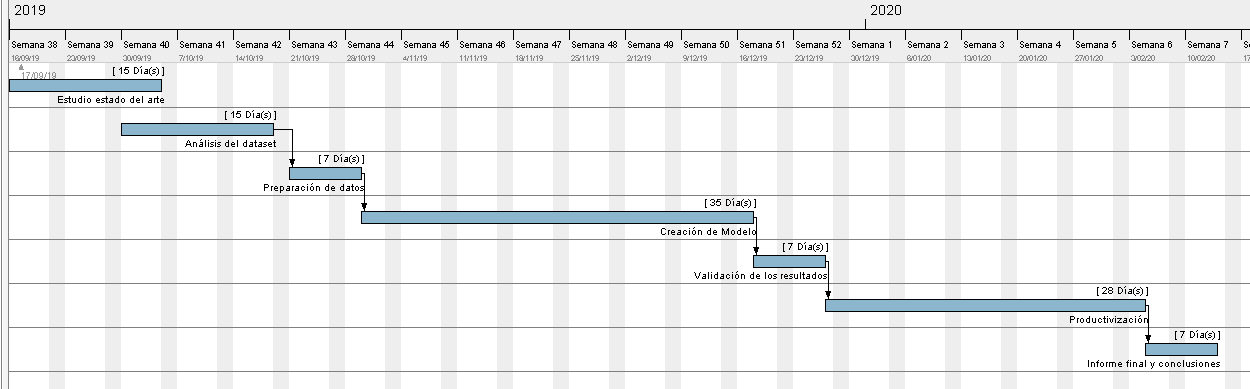
\includegraphics[width=\textwidth]{images/intro/gantt}
	\caption{Diagrama de Gantt}
	\label{fig:gantt}
\end{figure}


\begin{itemize}
	\item \textbf{Estudio estado del arte}: En esta fase se realizará una prospección para conocer el estado del arte en todos los puntos relacionados con el proyecto: Procesamiento del Lenguaje Natural, tecnologías de tratamiento de datos en tiempo real y \textit{Big Data}. 
	
	\item \textbf{Análisis del \textit{dataset}}: El propósito de esta tarea es entender el \textit{dataset}  y estudiar las posibilidades del mismo. 
	
	\item\textbf{ Preparación del \textit{dataset}}: Una vez realizado el estudio del \textit{dataset} es necesario realizar labores de limpieza y transformación de los datos de modo que estos datos sean válidos para nuestro objetivo.
	
	\item \textbf{Creación del modelo}: En esta fase se procederá a la creación de un modelo capaz de obtener los temas de los que habla una determinada llamada. Este modelo será el \textit{core} de nuestro proyecto.
	
	\item \textbf{Validación de los resultados}: Una vez entrenado el modelo será necesario validar los resultados obtenidos para poder evaluar la bondad de nuestro modelo. 
	
	\item\textbf{ Productivización}: El trabajo no acaba con la creación de un buen modelo que nos permita extraer los temas de nuestras llamadas. Este modelo tendrá que ser puesto en producción y permitir al usuario final extraer los temas de las llamadas en tiempo real y darle la opción de crear alarmas basadas en la variación del número de eventos (llamadas) de un determinado tema.
	\item\textbf{ Informe final y conclusiones}: Por último, una vez llevado a a producción nuestro modelo, se realizará un informe final donde, entre otros puntos, se evaluarán los resultados obtenidos y se extraerán conclusiones y pasos futuros.
\end{itemize} 

\begin{figure}[!ht]
	\centering
	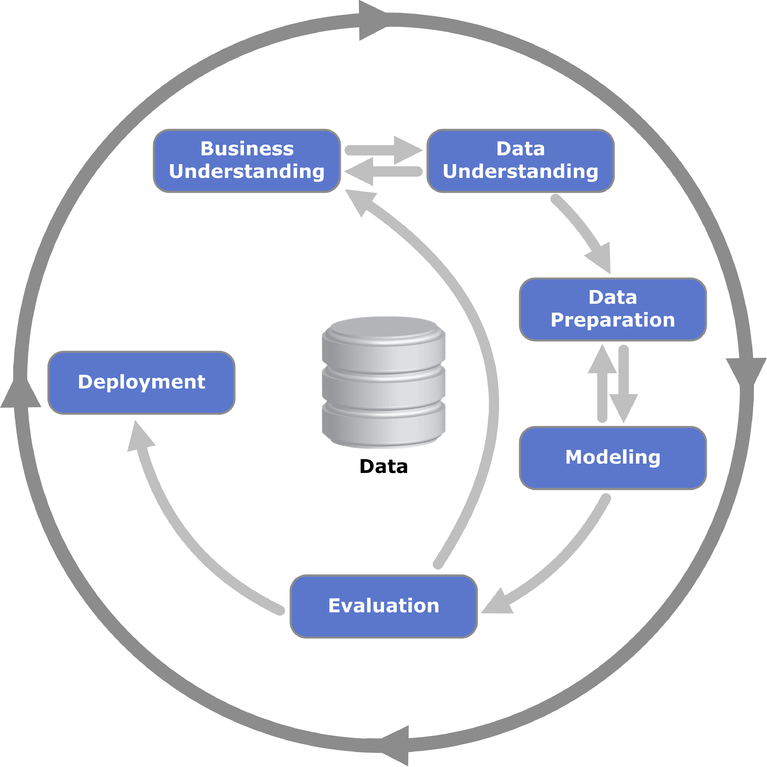
\includegraphics[width=0.63\textwidth]{images/intro/crispdm}
	\caption{Fases del modelo CRISP-DM}
	\label{fig:crispdm}
\end{figure}


Estas fases están basadas en el estándar \textbf{\textit{CRISP-DM}} (\cite{crispdm}), añadiendo una última tarea para nuestro informe final, \textit{CRISP-DM} nos proporciona una descripción del ciclo de vida de los proyectos de minería de datos de un modo bastante similar al que se aplica en los modelos de ciclo de vida de desarrollo \textit{software}.


 

En la Figura \ref{fig:crispdm} se observa el diseño de este modelo y cómo representa el ciclo de vida de un proyecto de minería de datos. En la imagen podemos ver en primer lugar un círculo exterior que refleja la naturaleza cíclica de los proyectos de minería de datos, además vemos cómo la secuencia de tareas no es rígida, pudiendo saltar hacia adelante o atrás entre tareas. En la gráfica se representan mediante flechas las dependencias más importantes y usuales entre tareas.

En nuestro desarrollo usaremos este modelo, aunque en el diagrama de la Figura \ref{fig:gantt} aparezca una secuencia de tareas más rígida, será usual, por ejemplo, el salto recíproco entre las fases de preparación de los datos y creación del modelo.



\chapter{Estado del Arte}
\label{chapter:estadoarte}


El objetivo de este apartado es hacer un recorrido por el estado del arte relacionado con el proyecto, este recorrido lo enfocaremos desde tres puntos de vista diferentes:
\begin{itemize}
	\item \textbf{Procesamiento del Lenguaje Natural}: En este apartado nos centraremos en el procesamiento del lenguaje natural y su evolución a lo largo del tiempo. 
	\item \textbf{\textit{Deep Learning} y aplicación al Procesamiento del Lenguaje Natural}: En la segunda parte pondremos foco en el \textit{Deep Learning}, sus ventajas y cómo se están aplicando estos métodos al procesamiento de lenguaje natural. 
	\item \textbf{\textit{Big Data} y \textit{Fast Data}}: Por último, haremos un repaso a la evolución del \textit{Big Data} y cómo la tendencia actual es realizar el procesamiento en tiempo real mediante \textit{Fast Data}.
\end{itemize}

\section{Procesamiento de lenguaje natural}

\subsection{Historia}

Para hablar de los orígenes del procesamiento del lenguaje natural (a partir de ahora NLP por sus siglas en inglés \textit{Natural Lenguage Processing}) tal y como lo conocemos, tendríamos que remontarnos a los años 50, concretamente al artículo ``\textit{Computing Machinery and Intelligence}'' escrito por Alan Turing \cite{turing_1950}. En este artículo aparece el NLP dentro del campo de la inteligencia artificial y se presenta por primera vez el conocido ``Test de Turing`''. Este test convirtió la pregunta abstracta de ``¿Son capaces de pensar las máquinas?'' en un juego llamado: ``\textit{The Imitation Game}''. El juego propuesto inicialmente, de forma muy resumida, consiste en ver si una persona (interrogador) interrogando a dos personas (un hombre y una mujer), era capaz de descubrir el sexo de cada una; la modificación del mismo sustituye las dos personas de distinto sexo por una persona y una máquina y el interrogador debe ser capaz de descubrir si las preguntas están siendo respondidas por un humano o una máquina. En el caso de que no sepa discernir, la computadora gana la partida. Podemos encontrar más información al respecto en el libro \cite{turing}.



A partir de los avances de Turing y hasta los 80 el crecimiento en el campo del NLP se produjo principalmente con la creación de complejos sistemas basados en reglas escritas a mano. Fue en esta década cuando empezamos a vivir la incorporación de algoritmos de \textit{machine learning} enfocados al procesamiento del lenguaje natural. Este hecho se vio motivado principalmente por el increíble avance en la capacidad de cómputo, ya predicho por la ley de Moore, y por la aplicación de teorías ya existentes como los trabajos de Chomsky. 


Desde el comienzo de la aplicación de modelos de \textit{machine learning}, y de nuevo motivados por el crecimiento de la capacidad computacional de los sistemas actuales, se ha pasado de utilizar árboles de decisión, que creaban de manera automática reglas similares a las que se venían creando manualmente, a los modelos de \textit{deep learning} que están en auge en la última década. 

\subsection{Aplicaciones}

En el apartado anterior hicimos referencia a ``\textit{The Imitation Game}'' como inicio de lo que hoy conocemos como procesamiento de lenguaje natural, sin embargo, las aplicaciones en este campo han crecido de forma vertiginosa en estos 70 años, principalmente en las últimas décadas. Hoy en día, si tuviéramos que contestar a la pregunta: ``¿son capaces de pensar las máquinas?'', implicaría algo más que superar el test de Turing. Mirando a nuestro alrededor nos encontraríamos con asistentes de voz como Alexa o Siri que no solo contestan a nuestras preguntas, si no que realizan un trabajo de pasar nuestra voz a texto (\textit{Speech to Text}) y de nuevo el texto resultante a voz (\textit{Text to Speech}). Nos encontraríamos también con sistemas capaces de realizar traducciones simultáneas, otros capaces de autocompletar textos, de identificar preguntas y respuestas, de clasificar textos de acuerdo a temas o autores, incluso de analizar sentimientos positivos o negativos teniendo como entrada un texto u opinión... 


Según \cite{goldberg_2017} todos estos problemas tan diversos podríamos clasificarlos según en el punto del análisis que nos centremos: 

\begin{itemize}
	\item \textbf{Análisis de palabras}: En este tipo de problemas se pone foco en las palabras, como pueden ser ``perro'', ``hablar'', ``piedra'' y necesitamos decir algo sobre ellas. Por ejemplo: ``¿estamos hablando de un ser vivo?'', ``¿a qué lenguaje pertenece?'', ``¿cuáles son sus sinónimos o antónimos?''. Actualmente este tipo de problemas son menos frecuentes, ya que normalmente no pretendemos analizar palabras aisladas sino que es preferible basarse en un contexto. 
	
	\item \textbf{Análisis de textos}:  En este tipo de problemas no trabajamos solo con palabras aisladas, sino que disponemos de una pieza de texto que puede ser una frase, un párrafo o un documento completo y tenemos que decir algo sobre él. Por ejemplo: ``¿se trata de spam?'', ``¿qué tipo de texto es?'', ``¿el tono es positivo o negativo?'', ``¿quién es su autor?''.Este tipo de problemas son muy comunes y nos vamos a referir a ellos como \textbf{problemas de clasificación de documentos}.   
	
	\item \textbf{Análisis de textos pareados}: En esta clase de análisis disponemos de  dos textos (también podrían ser palabras aisladas) y tenemos que decir algo sobre ellos. Por ejemplo, ``¿los textos son del mismo autor?'', ``¿son pregunta y respuesta?'', ``¿son sinónimos?'' (para el caso de palabras aisladas).
	
	\item \textbf{Análisis de palabras en contexto}: En estos casos de uso, a diferencia del primer análisis que trataba unicamente con  palabras aisladas, tenemos que clasificar una palabra en particular en función del contexto en el que se encuentra. 
	
	\item \textbf{Análisis de relación entre palabras}: Este último tipo de análisis tiene como objetivo deducir la relación entre dos palabras existentes en un documento. 
	
\end{itemize}

Dependiendo del problema que queramos abordar usaremos un tipo de características del lenguaje u otro, por ejemplo, es usual que si estamos analizando palabras aisladas nos centremos en las letras de una palabra, sus prefijos o sufijos, su longitud, la información léxica extraída de diccionarios como \textit{WordNet} \cite{wordnet}, etc. En cambio, si estamos trabajando con texto, lo normal es que nos fijemos en otros conceptos estadísticos como el histograma de las palabras dentro del texto, ratio de palabras cortas vs largas, número de veces que aparece una palabra en un texto comparado con el resto de textos...  

El proyecto que se presenta en este documento está centrado en el análisis de textos, concretamente en extraer los temas de un documento (o llamada). Este tipo de problemas se conoce como modelización de \textit{topics}. 

En el siguiente punto de este apartado nos centraremos en algunos modelos y avances en este área que puedan servirnos de apoyo para nuestro proyecto. 


\subsection{Modelización de temas}
La modelización de topics hace referencia a un grupo de algoritmos de \textit{machine learning} que infieren la estructura latente existente en un grupo de documentos. 

Aunque la mayoría de los algoritmos de modelización son no supervisados, al igual que los algoritmos tradicionales de \textit{clustering}, existen también algunas variantes supervisadas que necesitan disponer de documentos etiquetados. 

Quizás el algoritmo más conocido para la modelización de topics sea el \textit{Latent Dirichlet Allocation} (normalmente conocido por su acrónimo, LDA). LDA fué presentado en 2003 en el artículo \cite{Blei_LDA}. Este algoritmo no supervisado asume que cada documento es una distribución probabilística de \textit{topics} y cada \textit{topic}, a su vez, es una distribución de palabras del documento. LDA usa una aproximación llamada ``\textit{bag of words}'', en la que cada documento es tratado como un vector con el conteo de las palabras que aparecen en el mismo. La principal característica de LDA es que la colección de documentos comparten los mismos topics, pero cada documento contiene esos topics en una proporción diferente. 


A partir de LDA surgieron numerosas variantes que repasaremos de forma breve, por ejemplo, en el mismo año de la creación de LDA y también presentado por los mismos autores en \cite{Blei_HTM}, surgió una \textbf{variante jerárquica} que permitía representar los \textit{topics} jerarquicamente. En 2006 en \cite{Blei_DTM} se desarrolla un modelo LDA dinámico denominado DTM (\textit{Dinamic Topic Model}), en el que se introduce la variable temporal y los \textit{topics} pueden ir cambiando a lo largo del tiempo. En el artículo \cite{Blei_CTM} nos encontramos con otra variante de LDA llamada CTM (\textit{Correlated topic model}) que nos permite encontrar correlaciones entre \textit{topics}, ya que algunos temas es probable que sean más similares entre sí. Por último, nos encontramos con una variante de LDA denominada ATM (\textit{Author-Topic Model}) propuesta  por	Michal Rosen-Zvi en su artículo \cite{Rosen-Zvi_AMA_2010}  y desarrollada por el mismo en 2010, en la que los documentos son una distribución probabilística tanto de autores como de \textit{topics}.    


Podemos encontrar un resumen más completo del estado del arte en cuanto a la modelización de \textit{topics} en el artículo \cite{Mahmood2013LiteratureSO}. 

\section{Deep Learning  y aplicación al NLP}
El objetivo de esta sesión es entender el concepto de \textit{Deep Learning} y analizar el estado del arte del \textit{Deep Learning} aplicado al procesamiento del lenguaje natural. Para poder entender el \textit{Deep Learning} es conveniente entender los modelos de aprendizaje supervisados y saber qué provoca su aparición y popularidad de los últimos años. Posteriormente nos centraremos en los fundamentos del \textit{Deep Learning} para finalizar con las aplicaciones actuales en el ámbito del procesamiento del lenguaje natural y que nos sirvan de apoyo para la ejecución del proyecto.


\subsection{Aprendizaje supervisado}
El aprendizaje supervisado consiste en aprender una función a través de un conjunto de datos, llamados de entrenamiento, mediante la cual podamos obtener una salida a partir de una determinada entrada. Se espera que esta función, una vez realizado el entrenamiento, sea capaz de producir una salida correcta incluso para datos nunca vistos. Es muy habitual el uso de estos tipos de algoritmos para casos de clasificación y/o predicción. 

Buscar entre todas las posibles infinitas funciones posibles para encontrar la función que mejor se adapte a nuestro conjunto de datos es un trabajo inviable, es por ello que normalmente se realiza la búsqueda entre un conjunto de funciones limitadas. En un primer lugar, y hasta hace aproximadamente una década, los modelos más populares de aprendizaje supervisado fueron los modelos lineales, provenientes del mundo de la estadística, estos modelos son fáciles de entrenar, fáciles de interpretar y muy efectivos en la práctica. 

A partir de entonces, y motivado en parte por el aumento en las capacidades de cómputo, surgen otros modelos como las máquinas de vectores de soportes (\textit{Support Vector Machines}, SVMs) o las redes neuronales, en las que nos centraremos en el siguiente apartado.


\subsection{Deep Learning}
Dentro del \textit{Machine Learning} y usualmente relacionado con el aprendizaje supervisado, nos encontramos con un sub-campo denominado \textbf{Deep Learning} que utiliza las redes neuronales para la creación de modelos. Como su nombre indica las redes neuronales consisten en unidades de cómputo llamadas neuronas que están interconectadas entre sí. Una neurona es una unidad de cómputo que posee múltiples  entradas y una  salida, esta neurona multiplica cada entrada por un peso para posteriormente realizar una suma y, por último, aplicar una función de salida no lineal. Si los pesos se establecen correctamente y tenemos un número suficiente de neuronas, una red neuronal puede aproximar a un conjunto muy amplio de funciones matemáticas. 

En las redes neuronales, las neuronas suelen organizarse por capas que se encuentran conectadas entre sí. Mientras más capas tengamos más características podremos extraer de nuestros datos de entrada y podremos aproximar un mayor número de funciones (sin perder de vista el sobrentrenamiento). Hablamos que una red es profunda cuando contiene un gran número de capas, por ello el término de \textit{Deep Learning}. 





\subsection{Redes neuronales en NLP}% Podemos llamarle embedding o representación de palabras

Es usual, en el ámbito del reconocimiento de imágenes, utilizar información acerca de la dimensionalidad de las mismas. Este tipo de información nos permite extraer características  teniendo en cuenta los píxeles vecinos. Tradicionalmente, en el ámbito del procesamiento del lenguaje natural, esto no se ha llevado a cabo debido a que cada palabra (o n-grama) se trataba como una entidad aislada. 

En cambio, existe otro método de representar las palabras en el lenguaje natural que sí es capaz de captar la ``dimensionalidad'' de una forma similar a como lo realizamos en las imágenes. Este modo deja de tratar la palabra como un ente aislado y  es capaz de captar el significado de la misma, esta representación se denomina distribuida y consiste en convertir las palabras en vectores en los que cada dimensión capte características diferentes de las palabras. Este tipo de representaciones dará lugar a vectores similares para palabras semánticamente parecidas. 

Una de las soluciones más populares que nos permiten convertir una palabra a un vector (\textit{word2vec}) que contenga información de la palabra en función del contexto se detallan en el artículo \cite{word2vec} . Aquí se presentaron dos modelos llamados Skip-Gram y CBOW. Estos modelos utilizan redes neuronales para predecir una palabra en función de su contexto o el contexto en función de una palabra, el vector que se utiliza para representar la palabra es el vector de pesos de la capa oculta. 



\subsection{Arquitecturas especializadas}

Después de introducir las redes neuronales y el modo en el que podemos representar las palabras, frases o documentos para ser usados como entrada en nuestro modelo; vamos a centrarnos en comentar dos tipos de redes neuronales que se usan de manera tradicional en tareas de Procesamiento de Lenguaje Natural. 

Los dos tipos de redes neuronales que comentaremos son las redes neuronales convolucionales y las redes neuronales recurrentes. Haremos una introducción a cada una de ellas, comentaremos sus aplicaciones al PLN y sus ventajas y convenientes con respecto a otro tipo de métodos. 


\subsubsection{Redes neuronales convolucionales}

Las redes neuronales convolucionales (llamadas usualmente CNN, por su nombre en inglés \textit{\textbf{C}onvolutional \textbf{N}eural \textbf{N}etworks}) son un tipo de redes neuronales que deben su nombre a la operación matématica de convolución que realizan. Esta operación consiste en aplicar a una matriz de entrada multidimensional, un filtro o kernel también multidimensional y obtener una salida, también denominada mapa de características. En la figura \ref{fig:cnn1} podemos ver una representación gráfica de esta operación para un ejemplo de 2 dimensiones.

\begin{figure}[!ht]
	\centering
	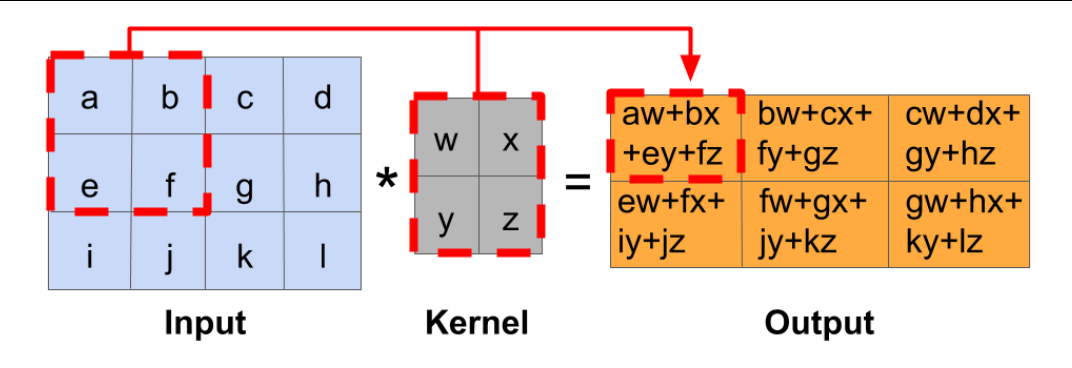
\includegraphics[width=0.7\textwidth]{images/arte/cnn1}
	\caption{Ejemplo de una convolución de dos dimensiones. Fuente \cite{temariodeeplearning}}
	\label{fig:cnn1}
\end{figure}


TODO Reduccion dimensión padding...

El proceso explicado anteriormente correspondería con una capa convolucional, que son el corazón de las redes neuronales convolucionales, sin embargo, en una red neuronal convolucional estas capas coexisten con otro tipo de capas que nos ayudaran a mejorar nuestros modelos. Las más usuales son:

\begin{itemize}
	\item Capa de agrupamiento (\textit{polling} en inglés): El objetivo de esta capa es agrupar un conjunto de salidas para obtener un único valor, al conjunto de valores de entrada (seleccionado de nuevo con un filtro) se le aplica una función para obtener un único valor. Aunque se pueden utilizar diferentes funciones, como puede ser la media, lo más usual es aplicar la función de máximo (\textit{max-polling}). Es habitual, intuir que usando esta función nos estamos quedando con las características más relevantes de cada cuadrante (del tamaño del filtro) de la entrada.
	\item Capa totalmente conectada: Hemos visto ejemplos de capas totalmente conectada al introducir las redes neuronales, esta capas usualmente se usan al final de nuestra red para tareas de clasificación, teniendo la última capa un número de neuronas igual al número de clases que pretendemos clasificar.
	\item Capa RELU: Si observamos la descripción de la operación de convolución nos damos cuenta de que se trata de una operación totalmente lineal, es por ello que después de cada capa de convolución es usual agregar una capa no lineal (también llamada capa de activación). Aunque se pueden utilizar otras funciones como la tangente o la función sigmoide, lo más usual es utilizar la función RELU.
	
	\item Capa de Dropout: 
	
\end{itemize}

En una red neuronal convolucional normalmente coexisten otro tipo de



TODO seguir con pooling ...

Encontramos una explicación más profunda sobre las redes convolucionales y su uso general en \cite{temariodeeplearning}. Nosotros nos centraremos en tener una visión general de su aplicación al Procesamiento del Lenguaje Natural, que también puede ampliarse en \cite{goldberg_2017}.


TODO palabras

\subsubsection{Redes neuronales recurrentes}


TODO explicación pros y contras

\section{BigData y Fast Data}

El primer uso del término  \textit{Big Data}  se da en un artículo de Michael Cox y David Ellsworth de la NASA publicado en 1997 (\cite{Cox_1997}), donde hacen referencia a la dificultad de procesar grandes volúmenes de datos con los métodos de la época. Sin embargo, fue en 2001 cuando encontramos la definición más conocida y aceptada de \textit{Big Data} hecha por el analista Laney Douglas en su artículo ``3D Data Management: Controlling Data Volume, Velocity y Variety''(\cite{laneay_2013}) en el que se hacía referencia a las ya ``famosas'' tres \textit{V}s:

\begin{itemize}
	\item \textbf{V}olumen:  Cada vez los volúmenes de datos son mayores.
	\item \textbf{V}elocidad: Es cada vez mayor la velocidad con la que se generan los datos.  
	\item \textbf{V}ariedad: Dejamos de tener únicamente datos completamente estructurados para trabajar con datos no estructurados y/o  semi-estructurados. 
\end{itemize} 


Google, como es obvio, también  se enfrentó a un importante problema a la hora de procesar la ingente cantidad de datos que generaba día a día y que no podían ser procesados de manera eficiente con el \textit{software} existente, es por ello que en el año 2003 presenta en \cite{GFS} su  \textit{``Google File System''} (GFS) y un año después \textit{Map Reduce} \cite{MapReduce}, estas dos capas de almacenamiento y procesamiento distribuido dieron lugar al nacimiento de lo que hoy conocemos como \textit{\textbf{Big Data}}.

Sin embargo, estas aportaciones no empezaron a tomar una repercusión relevante fuera de Google hasta el nacimiento del \textit{framework} Hadoop en 2006, un ecosistema con una gran cantidad de servicios pero cuya base fue Map Reduce y HDFS (basado en GFS). La complejidad del ecosistema \textit{Hadoop} hizo que éste no empezara a aparecer en las mayoría de las empresas hasta la creación de la compañía \textit{Cloudera} en 2009, que empezó a empaquetar los diferentes componentes del ecosistema \textit{Hadoop}, ofreciendo distribuciones estables y soporte para sus clientes. 

Durante estos 10 años la popularidad de \textit{Hadoop} ha crecido exponencialmente y junto con las BBDD NoSQL, nacidas también a partir de Google con su BigTable, forman lo que hoy conocemos como Big Data. 



El auge del \textbf{Big Data} ha llevado a algunas empresas a tener verdadera obsesión por el almacenamiento de todos los datos de sus clientes y las operaciones realizadas, creando inmensos \textit{datalakes} donde tener enormes históricos de todos sus datos, este ``síndrome de Diógenes digital'' creado por falsas expectativas, por la imposibilidad de extraer valor de los datos o por la dimensión cambiante de las empresas actuales, en la que los datos de años atrás pueden no ser relevantes en el presente, es uno de los posibles motivos por lo que el tratamiento de los datos esta cambiando. Otro de los motivos para el cambio de rumbo del \textit{Big Data} está relacionado con la \textit{V} de Velocidad, hoy en día no solo es importante la capacidad de ingestar rápidamente los datos, sino la capacidad de poder procesar y obtener decisiones o actuar en tiempo real a partir de los datos, aportando valor al negocio. En este escenario se vuelve más importante la velocidad que el volumen de datos, esto es lo que se denomina \textit{Fast Data}. 

Dentro del \textit{Fast Data} es habitual el uso de BBDD \textit{in-memory}, de buses de eventos y de tecnologías de procesamiento capaces de procesar los eventos en tiempo real. Como veremos posteriormente al desarrollar nuestra arquitectura, el \textit{Fast Data} será una parte fundamental en nuestro proyecto en el que tendremos que clasificar las llamadas en tiempo real y tomar decisiones (o alarmar) en función de las mismas.

\chapter{Arquitectura y tecnologías}
\label{chapter:arquitectura}

El objetivo de este capítulo es tener un diseño esquemático de la solución que se plantée, este diseño será abordado en primer lugar desde un punto de vista lógico, de acuerdo a las necesidades del proyecto, posteriormente aterrizaremos esta arquitectura con tecnologías concretas que nos ayuden a conseguir el objetivo deseado.

\section{Arquitectura}
\begin{figure}[!ht]
	\centering
	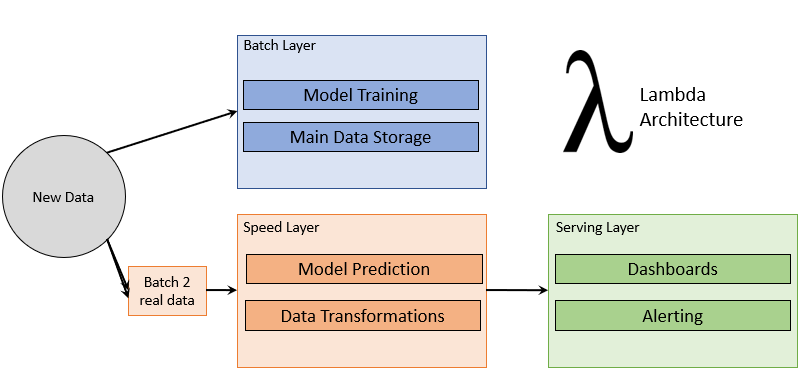
\includegraphics[width=1\textwidth]{images/arqu/lambda}
	\caption{Arquitectura Lambda propuesta}
	\label{fig:lambda}
\end{figure}




En este apartado definiremos la arquitectura desde un punto de vista lógico, esta arquitectura debe responder a los objetivos propuestos para cumplir con las necesidades de negocio existentes. 


En líneas generales, podemos ver la arquitectura de nuestro sistema como una arquitectura \textit{Lambda} en la que disponemos de una capa \textit{batch}, una capa rápida o \textit{real-time} y una última capa de servicio.



La capa batch será la encargada de entrenar el modelo a través de los datos de las llamadas, la capa rápida obtendrá los \textit{topics} de las llamadas en tiempo real usando el modelo previamente entrenado y por último la capa de servicio será la encargada de mostrar estos datos al usuario mediante cuadros de mando.  

En la figura \ref{fig:lambda} podemos ver un esquema general de nuestra arquitectura. A continuación definimos con más detalle cada una de las capas del modelo.




\subsection{Capa Batch}
El \textit{core} del proyecto que abordamos es el modelo, encargado de extraer los \textit{topics} de las transcripciones de llamadas al servicio de atención al cliente. Este modelo debe entrenarse usando un histórico suficientemente amplio. 

El modelo es un elemento vivo en nuestra arquitectura y, además de por posibles mejoras en los hiperparámetros o por la tecnología, debe re-entrenarse conforme se vayan recibiendo datos nuevos en el histórico, ya que es lógico pensar que la temática de las consultas variarán a lo largo del tiempo debido por ejemplo al lanzamiento de nuevos productos. 


\subsection{Capa Real-Time}
La \textit{speed layer} de nuestro proyecto será la encargada de recibir los datos en tiempo real, las llamadas serán publicadas en un bus de eventos y estos eventos serán consumidos por una capa de procesamiento que será la encargada de aplicar el modelo entrenado en la capa \textit{batch} a los nuevos datos. Los \textit{topics} resultantes de cada llamada serán publicados de nuevo en este bus para poder ser ingestados posteriormente a una BBDD NO-SQL, que será la encargada de proporcionar la información a la capa de servicio. 

Aprovecharemos también las características de la BBDD NoSQL para, mediante un módulo de \textit{Machine Learning}, detectar anomalías en series temporales y poder alarmar en el caso de que un \textit{topic} concreto se dispare en algún momento.  

Debido a la situación actual, las llamadas no se ingestan en \textit{real-time} si no que se procesan en mini \textit{batches} cada cierto tiempo. Es muy probable que este escenario cambie en el futuro por lo que se construirá un elemento de entrada a la capa rápida que transformará el mini-batch en eventos conforme vayan ejecutándose (este elemento puede observarse en la figura \ref{fig:lambda} como \textit{Batch 2 real data}). Esta pieza será suprimida una vez las llamadas sean recibidas en tiempo real. 


\subsection{Capa de Servicio}
Una vez almacenados los datos en la BBDD debemos construir un frontal que muestre al usuario el número de llamadas analizadas, el modelo utilizado y principalmente la evolución de los \textit{topics} a lo largo del tiempo. 

Lo ideal es que esta capa de servicio se vaya actualizando en tiempo cuasi-real y permita a los diferentes usuarios realizar cuadros de mando personalizados según sus necesidades. 

Otro requisito esencial en este tipo de proyectos es que la información este disponible vía API-REST para poder ser consumida por terceros.    


\section{Integración y Despliegue Continuos}
Como ya hemos visto al hablar del entrenamiento del modelo, el desarrollo de este tipo de proyectos no tiene un principio y un final, si no que se trata de un proceso cíclico en el que por necesidades del negocio, por cambio en los datos o por cambio en la tecnologías, será necesario añadir mejoras o modificaciones en nuestro desarrollo. 

Por estos motivos es conveniente definir mecanismos que nos permitan, tras cada cambio efectuado, poder realizar las pruebas necesarias y desplegar estos cambios de una manera totalmente automatizada y sin intervención del usuario. 

Aunque este apartado queda fuera de la implementación inicial del proyecto es imprescindible llevarlo a cabo para que este sea sostenible a lo largo del tiempo. 


TODO (Posible ampliar con apuntes sobre el ciclo de vida de los datos y contar beneficios de un despliegue continuo)

\section{Tecnologías}

Al igual que la arquitectura descrita anteriormente era la encargada de responder a las necesidades de negocio, las tecnologías descritas en este apartado nos darán las piezas necesarias para poder construir esa arquitectura y dar respuesta a nuestro caso de uso. 


En el proceso de selección de las tecnologías, no solo se ha tenido en cuenta la idoneidad de las mismas para el caso de uso, si no que se ha valorado también la experiencia en la misma y la disponibilidad dentro del entorno de trabajo. Esto puede provocar que en algunos casos aunque la tecnología se adapte al caso de uso, puedan existir otras soluciones más óptimas cuyo uso era menos viable dado los plazos de ejecución del proyecto. 

A continuación enumeraremos las tecnologías agrupadas en las diferentes capas que hemos comentado en el apartado de arquitectura, además añadiremos las tecnologías que se usarán para la integración y despliegue continuo. 

\subsection{Capa batch}

\begin{itemize}
	\item \textbf{Spark}: Es un framework de computación en clúster. Este \textit{framework} se encuentra desplegado sobre un clúster Hadoop, específicamente una distribución HortonWorks, y posee librerías específicas para Machine Learning como MLLIB.
	\item \textbf{Tensorflow} sobre GPUs: Para el entrenamiento de los modelos también disponemos de un cluster con GPUs sobre el que podremos correr código usando la librería de Google Tensorflow para entrenar nuestros modelos.
\end{itemize}

\subsection{Capa Real-Time}

\begin{itemize}
	\item \textbf{Kafka}: Es el \textit{core} de la capa rápida, se trata de un bus de evento distribuido a través del cual se realizara la ingesta o publicación de los eventos (llamadas). Las diferentes capas de procesamiento que requieran estos eventos se suscribirán a este Bus.
	\item \textbf{Microservicios}: En nuestra capa Real Time construiremos diferentes microservicios en la capa de procesamiento, estos microservicios serán por ejemplo los encargados de devolver los \textit{topics} de cada llamada a partir de una llamada API REST. Estos microservicios correran sobre contenedores en una plataforma Openshift. 
	\item\textbf{ Kafka Stream y KSQL}: A la hora de procesar la información en eventos ingestada en nuestro Bus Kafka disponemos de dos herramientas muy potentes que son Kafka Stream y KSQL. El primero consiste en una serie de librerías que nos permiten construir aplicaciones y microservicios cuyo origen y destino sean un Bus Kafka. KSQL en cambio es un motor SQL aplicable a eventos que nos llegan mediante \textit{streaming}.
	\item \textbf{Logstash}: Una vez hayamos extraído los \textit{topics} correspondientes a cada llamada o evento, tendremos que ingestar esta información en nuestra BBDD, que en este caso será Elasticsearch. Logstash nos permitirá leer de Kafka, realizar las transformaciones necesarias y volcar la información resultante en Elasticsearch.
	\item \textbf{Elasticsearch}: Aunque no se trata en el sentido más estricto de una BBDD No-SQL, si no de un motor de búsqueda, Elasticsearch nos permite almacenar la información en forma de documentos json y realizar consultas y agregaciones sobre cualquier campo. Entre las características que podemos aprovechar de Elasticsearch para nuestro objetivo están: 
	\begin{itemize}
		\item Ingesta en tiempo casi real.
		\item Consulta en tiempo casi real. 
		\item Disponibilidad de mecanismos de ingesta (Logstash) y consulta (kibana).
		\item Posibilidad de crear alarmas en base a consultas. 
		\item Posibilidad de crear \textit{jobs} de Machine Learning que detecten anomalías en series temporales. 
	\end{itemize}
	
	
\end{itemize}

\subsection{Capa Servicio}
\begin{itemize}
	\item \textbf{Elasticsearch API REST}: Toda la información almacenada previamente en Elasticsearch puede ser accedida a través de su API REST por lo que será nuestro método de publicación de la información. 
	\item \textbf{Kibana}: Será el frontal donde los usuarios podrán consultar sus diferentes cuadros de mando y construir nuevos de acuerdo a sus necesidades. También, gracias al modulo de \textit{machine learning} de Elasticsearch, los usuarios podrán crear \textit{jobs} de \textit{machine learning} para detectar anomalías en los temas tratados y generar las alertas necesarias.
\end{itemize}


\subsection{Integración y Despliegue Continuo}
Aunque la implementación de esta parte se escapa de los plazos del proyecto, las tecnologías que se usarán para llevarla a cabo serán. 
\begin{itemize}
	\item \textbf{BitBucket}: Será el repositorio usado para almacenar las nuevas versiones de nuestro \textit{software} de manera que podamos tener un control de versiones.
	\item \textbf{Jenkins}: Es un servidor de integración continua \textit{open source}  que mediante la creación de tareas nos ayudará a realizar el \textit{build} de nuestro software realizando de manera automática las pruebas necesarias.
\end{itemize}

\part{Modelado: datos, modelos y optimizaciones}
\chapter{Conjunto de datos}
\label{chapter:dataset}
El primer paso cuando nos enfrentamos a un problema de minería de datos es comprender los datos con los que contamos y ver si se adaptan a nuestras necesidades. En este caso, al tratarse de un proyecto que se realiza dentro de una empresa, tenemos la posibilidad de acudir a las áreas dueñas del dato para solicitarle información adicional sobre el mismo. 

En este apartado haremos un recorrido 



\section{Evolución del \textit{dataset}}

\subsection{Las llamadas}

Durante este apartado hemos realizado un análisis del conjunto de datos más completo que teníamos hasta la fecha, no obstante, el proceso para conseguir y entender este conjunto de datos no ha sido una tarea trivial sino que se ha tratado de un proceso iterativo en el que ha sido necesario involucrar a varias áreas y extraer información de diversas fuentes de datos de la compañía. Estos datos, como veremos de nuevo en el siguiente capítulo, nos han llevado a crear modelos poco eficientes que nos han situado otra vez en el punto de partida. 

Aunque el hecho de volver a la fase de recopilación y entendimiento de los datos es algo que ya preveíamos cuando presentamos el estándar \textbf{\textit{CRISP-DM}} (apartado \ref{section:intro:planificacion}) vamos a utilizar esta sección una breve muestra de los análisis iniciales para que pueda compararse con el análisis final y quede patente la evolución de los datos.



Este análisis fue realizado en \textit{PySpark} y el primer paso, como es obvio, fue cargar los datos en un \textit{dataframe} y comprobar la estructura del mismo: 


\vspace{0.5cm}

\begin{tcolorbox}[breakable, size=fbox, boxrule=1pt, pad at break*=1mm,colback=cellbackground, colframe=cellborder]
\prompt{In}{incolor}{1}{\boxspacing}
\begin{Verbatim}[commandchars=\\\{\}]
\PY{n}{domo\PYZus{}dataset} \PY{o}{=} \PY{n}{sqlContext}\PY{o}{.}\PY{n}{read}\PY{o}{.}\PY{n}{parquet}\PY{p}{(}\PY{l+s+s2}{\PYZdq{}}\PY{l+s+s2}{dataset/domo\PYZus{}dataset.parquet}\PY{l+s+s2}{\PYZdq{}}\PY{p}{)}
\PY{n}{domo\PYZus{}dataset}
\end{Verbatim}
\end{tcolorbox}

 \begin{tcolorbox}[breakable, size=fbox, boxrule=.5pt, pad at break*=1mm, opacityfill=0]
\prompt{Out}{outcolor}{1}{\boxspacing}
\begin{Verbatim}[commandchars=\\\{\}]
DataFrame[co\_llamada\_verint: string, id\_descarga:string,nu\_telefono\_actuacion:string, it\_llamada: timestamp, nu\_llamada\_ic: string, co\_grabacion: string,raw\_verint:array<string>, \_\_index\_level\_0\_\_: bigint]
\end{Verbatim}
\end{tcolorbox}


De los campos listados unicamente es factible extraer información del texto de la llamada (``raw\_verint''). El siguiente paso fue comprobar el número de llamadas que no contenían una transcripción nula. Además reparticionamos los datos y los dejamos en caché para realizar un análisis más eficiente: 

\vspace{0.5cm}


    \begin{tcolorbox}[breakable, size=fbox, boxrule=1pt, pad at break*=1mm,colback=cellbackground, colframe=cellborder]
\prompt{In}{incolor}{2}{\boxspacing}
\begin{Verbatim}[commandchars=\\\{\}]
\PY{n}{raw\PYZus{}verint} \PY{o}{=} \PY{n}{domo\PYZus{}dataset}\PY{o}{.}\PY{n}{select}\PY{p}{(}\PY{l+s+s2}{\PYZdq{}}\PY{l+s+s2}{raw\PYZus{}verint}\PY{l+s+s2}{\PYZdq{}}\PY{p}{)}\PY{o}{.}\PY{n}{rdd}\PY{o}{.}\PY{n}{filter}\PY{p}{(}\PY{k}{lambda} \PY{n}{x}\PY{p}{:} \PY{n}{x}\PY{p}{[}\PY{l+s+s2}{\PYZdq{}}\PY{l+s+s2}{raw\PYZus{}verint}\PY{l+s+s2}{\PYZdq{}}\PY{p}{]} \PY{o+ow}{is} \PY{o+ow}{not} \PY{k+kc}{None}\PY{p}{)}\PYZbs{}
    \PY{o}{.}\PY{n}{map}\PY{p}{(}\PY{k}{lambda} \PY{n}{x}\PY{p}{:} \PY{l+s+s2}{\PYZdq{}}\PY{l+s+s2}{ }\PY{l+s+s2}{\PYZdq{}}\PY{o}{.}\PY{n}{join}\PY{p}{(}\PY{n+nb}{map}\PY{p}{(}\PY{k}{lambda} \PY{n}{y}\PY{p}{:} \PY{l+s+s2}{\PYZdq{}}\PY{l+s+s2}{ }\PY{l+s+s2}{\PYZdq{}}\PY{o}{.}\PY{n}{join}\PY{p}{(}\PY{n}{y}\PY{p}{)}\PY{p}{,} \PY{n}{x}\PY{p}{)}\PY{p}{)}\PY{p}{)}\PYZbs{}
    \PY{o}{.}\PY{n}{repartition}\PY{p}{(}\PY{l+m+mi}{17}\PY{p}{)}
\PY{n}{raw\PYZus{}verint}\PY{o}{.}\PY{n}{cache}\PY{p}{(}\PY{p}{)}
\PY{n+nb}{print}\PY{p}{(}\PY{l+s+s1}{\PYZsq{}}\PY{l+s+s1}{Llamadas disponibles : }\PY{l+s+si}{\PYZob{}:,\PYZcb{}}\PY{l+s+s1}{\PYZsq{}}\PY{o}{.}\PY{n}{format}\PY{p}{(} \PY{n}{raw\PYZus{}verint}\PY{o}{.}\PY{n}{count}\PY{p}{(}\PY{p}{)}\PY{p}{)}\PY{p}{)}  
\end{Verbatim}
\end{tcolorbox}

    \begin{Verbatim}[commandchars=\\\{\}]
Llamadas disponibles : 185,109
    \end{Verbatim}
    
    
 A través de todas las llamadas obtuvimos una lista de palabras: 
    \vspace{0.5cm}
    
        \begin{tcolorbox}[breakable, size=fbox, boxrule=1pt, pad at break*=1mm,colback=cellbackground, colframe=cellborder]
    \prompt{In}{incolor}{3}{\boxspacing}
    \begin{Verbatim}[commandchars=\\\{\}]
    \PY{n}{raw\PYZus{}list\PYZus{}word} \PY{o}{=} \PY{n}{raw\PYZus{}verint}\PY{o}{.}\PY{n}{map}\PY{p}{(} \PY{k}{lambda} \PY{n}{document}\PY{p}{:} \PY{n}{document}\PY{o}{.}\PY{n}{strip}\PY{p}{(}\PY{p}{)}\PY{o}{.}\PY{n}{lower}\PY{p}{(}\PY{p}{)}\PY{p}{)} \PYZbs{}
                    \PY{o}{.}\PY{n}{map}\PY{p}{(} \PY{k}{lambda} \PY{n}{document}\PY{p}{:} \PY{n}{re}\PY{o}{.}\PY{n}{split}\PY{p}{(}\PY{l+s+s2}{\PYZdq{}}\PY{l+s+s2}{ }\PY{l+s+s2}{\PYZdq{}}\PY{p}{,} \PY{n}{document}\PY{p}{)}\PY{p}{)}
    
    \PY{n}{raw\PYZus{}list\PYZus{}word}\PY{o}{.}\PY{n}{take}\PY{p}{(}\PY{l+m+mi}{1}\PY{p}{)}
    \end{Verbatim}
    \end{tcolorbox}
    
    
    
Y eliminamos las \textit{Stopwords} en español usando el paquete \textit{ntlk}.

\vspace{0.5cm}
    
        \begin{tcolorbox}[breakable, size=fbox, boxrule=1pt, pad at break*=1mm,colback=cellbackground, colframe=cellborder]
    \prompt{In}{incolor}{4}{\boxspacing}
    \begin{Verbatim}[commandchars=\\\{\}]
    \PY{n}{StopWords} \PY{o}{=} \PY{n}{stopwords}\PY{o}{.}\PY{n}{words}\PY{p}{(}\PY{l+s+s2}{\PYZdq{}}\PY{l+s+s2}{spanish}\PY{l+s+s2}{\PYZdq{}}\PY{p}{)}
    
    \PY{n}{raw\PYZus{}no\PYZus{}stop} \PY{o}{=} \PY{n}{raw\PYZus{}verint}\PY{o}{.}\PY{n}{map}\PY{p}{(} \PY{k}{lambda} \PY{n}{document}\PY{p}{:} \PY{n}{document}\PY{o}{.}\PY{n}{strip}\PY{p}{(}\PY{p}{)}\PY{o}{.}\PY{n}{lower}\PY{p}{(}\PY{p}{)}\PY{p}{)} \PYZbs{}
    	\PY{o}{.}\PY{n}{map}\PY{p}{(} \PY{k}{lambda} \PY{n}{document}\PY{p}{:} \PY{n}{re}\PY{o}{.}\PY{n}{split}\PY{p}{(}\PY{l+s+s2}{\PYZdq{}}\PY{l+s+s2}{ }\PY{l+s+s2}{\PYZdq{}}\PY{p}{,} \PY{n}{document}\PY{p}{)}\PY{p}{)} \PYZbs{}
        \PY{o}{.}\PY{n}{map}\PY{p}{(} \PY{k}{lambda} \PY{n}{word}\PY{p}{:} \PY{p}{[}\PY{n}{x} \PY{k}{for} \PY{n}{x} \PY{o+ow}{in} \PY{n}{word} \PY{k}{if} \PY{n}{x} \PY{o+ow}{not} \PY{o+ow}{in} \PY{n}{StopWords}\PY{p}{]}\PY{p}{)}
    \PY{n}{raw\PYZus{}no\PYZus{}stop}\PY{o}{.}\PY{n}{take}\PY{p}{(}\PY{l+m+mi}{1}\PY{p}{)}
    \end{Verbatim}
    \end{tcolorbox}
    
       Volvemos a unir las palabras de la lista (ahora sin las \textit{stopwords}) para mostrar una nube de  palabras más frecuentes
    
        \begin{tcolorbox}[breakable, size=fbox, boxrule=1pt, pad at break*=1mm,colback=cellbackground, colframe=cellborder]
    \prompt{In}{incolor}{5}{\boxspacing}
    \begin{Verbatim}[commandchars=\\\{\}]
    \PY{n}{list\PYZus{}words} \PY{o}{=} \PY{n}{raw\PYZus{}no\PYZus{}stop}\PY{o}{.}\PY{n}{reduce}\PY{p}{(}\PY{k}{lambda} \PY{n}{a}\PY{p}{,}\PY{n}{b}\PY{p}{:} \PY{n+nb}{list}\PY{p}{(}\PY{n+nb}{set}\PY{p}{(}\PY{n}{a}\PY{o}{+}\PY{n}{b}\PY{p}{)}\PY{p}{)}\PY{p}{)}  
    \PY{n}{wordcloud} \PY{o}{=} \PY{n}{WordCloud}\PY{p}{(}\PY{p}{)}\PY{o}{.}\PY{n}{generate}\PY{p}{(}\PY{l+s+s2}{\PYZdq{}}\PY{l+s+s2}{ }\PY{l+s+s2}{\PYZdq{}}\PY{o}{.}\PY{n}{join}\PY{p}{(}\PY{n}{list\PYZus{}words}\PY{p}{)}\PY{p}{)}
    \PY{n}{plt}\PY{o}{.}\PY{n}{figure}\PY{p}{(}\PY{n}{figsize} \PY{o}{=} \PY{p}{(}\PY{l+m+mi}{20}\PY{p}{,}\PY{l+m+mi}{20}\PY{p}{)}\PY{p}{)}
    \PY{n}{plt}\PY{o}{.}\PY{n}{imshow}\PY{p}{(}\PY{n}{wordcloud}\PY{p}{,} \PY{n}{interpolation}\PY{o}{=}\PY{l+s+s1}{\PYZsq{}}\PY{l+s+s1}{bilinear}\PY{l+s+s1}{\PYZsq{}}\PY{p}{)}
    \PY{n}{plt}\PY{o}{.}\PY{n}{axis}\PY{p}{(}\PY{l+s+s2}{\PYZdq{}}\PY{l+s+s2}{off}\PY{l+s+s2}{\PYZdq{}}\PY{p}{)}
    \PY{n}{plt}\PY{o}{.}\PY{n}{show}\PY{p}{(}\PY{p}{)}
    \end{Verbatim}
    \end{tcolorbox}
    
      \begin{figure}[!ht]
                    	\centering
                    	\adjustimage{max size={0.9\linewidth}{0.9\paperheight}}{images/data/malo_wordclod1}
                    	\caption{Primeros datos: \textit{wordcloud} inicial}
                    	\label{fig:wordcloudmalo1}
                    \end{figure}
              
              
Como podemos observar en la nube de palabras obtenida, el resultado no fue el esperado. Las llamadas que aparecían no eran significante y entre ellas existían muchas malas  transcripciones. A partir de aquí intentamos abordar distintas aproximaciones que nos permitieran poder extraer algo de valor de los datos.

Un ejemplo de estas aproximaciones fue \textit{taggear} las palabras en  función de su categoría gramatical para quedarnos solo con una lista de candidatos. Para hacerlo de un modo eficiente de manera distribuida en promer lugar creamos un diccionario con las categorías y la raíz de las palabras: 

          
\vspace{0.5cm}
          
              \begin{tcolorbox}[breakable, size=fbox, boxrule=1pt, pad at break*=1mm,colback=cellbackground, colframe=cellborder]
          \prompt{In}{incolor}{6}{\boxspacing}
          \begin{Verbatim}[commandchars=\\\{\}]
          \PY{n}{tagger} \PY{o}{=} \PY{n}{treetaggerwrapper}\PY{o}{.}\PY{n}{TreeTagger}\PY{p}{(}\PY{n}{TAGLANG}\PY{o}{=}\PY{l+s+s1}{\PYZsq{}}\PY{l+s+s1}{es}\PY{l+s+s1}{\PYZsq{}}\PY{p}{,} \PY{n}{TAGPARFILE}\PY{o}{=}\PY{l+s+s2}{\PYZdq{}}\PY{l+s+s2}{/tmp/tree/spanish.par}\PY{l+s+s2}{\PYZdq{}}\PY{p}{,} \PY{n}{TAGDIR}\PY{o}{=}\PY{l+s+s2}{\PYZdq{}}\PY{l+s+s2}{/tmp/tree/tree\PYZhy{}tagger\PYZhy{}3.2.1/}\PY{l+s+s2}{\PYZdq{}}\PY{p}{)}          
          \PY{n}{vocabulary} \PY{o}{=}  \PY{n}{raw\PYZus{}no\PYZus{}stop}\PY{o}{.}\PY{n}{filter}\PY{p}{(}\PY{k}{lambda} \PY{n}{x}\PY{p}{:} \PY{n+nb}{len}\PY{p}{(}\PY{n}{x}\PY{p}{)}\PY{o}{\PYZgt{}}\PY{l+m+mi}{0}\PY{p}{)} \PYZbs{}
              \PY{o}{.}\PY{n}{flatMap}\PY{p}{(}\PY{k}{lambda} \PY{n}{document}\PY{p}{:} \PY{n}{document}\PY{p}{)} \PYZbs{}
              \PY{o}{.}\PY{n}{map}\PY{p}{(}\PY{k}{lambda} \PY{n}{word}\PY{p}{:} \PY{p}{(}\PY{n}{word}\PY{p}{,} \PY{l+m+mi}{1}\PY{p}{)}\PY{p}{)} \PYZbs{}
              \PY{o}{.}\PY{n}{reduceByKey}\PY{p}{(} \PY{k}{lambda} \PY{n}{x}\PY{p}{,}\PY{n}{y}\PY{p}{:} \PY{n}{x} \PY{o}{+} \PY{n}{y}\PY{p}{)}   \PYZbs{}
              \PY{o}{.}\PY{n}{map}\PY{p}{(}\PY{k}{lambda} \PY{n+nb}{tuple}\PY{p}{:} \PY{n+nb}{tuple}\PY{p}{[}\PY{l+m+mi}{0}\PY{p}{]}\PY{p}{)} 
          \PY{n}{vocabulary}\PY{o}{.}\PY{n}{cache}\PY{p}{(}\PY{p}{)}
          \PY{n}{vocabulary}\PY{o}{.}\PY{n}{count}\PY{p}{(}\PY{p}{)}
          \PY{n}{vocabulary\PYZus{}tags} \PY{o}{=} \PY{n+nb}{list}\PY{p}{(}\PY{n+nb}{map}\PY{p}{(}\PY{k}{lambda} \PY{n}{el}\PY{p}{:} \PY{p}{(}\PY{n}{el}\PY{p}{[}\PY{l+m+mi}{0}\PY{p}{]}\PY{p}{,} \PY{p}{(}\PY{n}{el}\PY{p}{[}\PY{l+m+mi}{1}\PY{p}{]}\PY{p}{,} \PY{n}{el}\PY{p}{[}\PY{l+m+mi}{2}\PY{p}{]}\PY{p}{)} \PY{p}{)} \PY{p}{,}\PY{n+nb}{map}\PY{p}{(}\PY{k}{lambda} \PY{n}{y}\PY{p}{:} \PY{n}{y}\PY{o}{.}\PY{n}{split}\PY{p}{(}\PY{l+s+s2}{\PYZdq{}}\PY{l+s+se}{\PYZbs{}t}\PY{l+s+s2}{\PYZdq{}}\PY{p}{)}\PY{p}{,}\PY{n+nb}{list}\PY{p}{(}\PY{n}{tagger}\PY{o}{.}\PY{n}{tag\PYZus{}text}\PY{p}{(}\PY{p}{(}\PY{l+s+s2}{\PYZdq{}}\PY{l+s+s2}{ }\PY{l+s+s2}{\PYZdq{}}\PY{o}{.}\PY{n}{join}\PY{p}{(}\PY{n}{vocabulary}\PY{o}{.}\PY{n}{collect}\PY{p}{(}\PY{p}{)}\PY{p}{)}\PY{p}{)} \PY{p}{)}\PY{p}{)}\PY{p}{)}\PY{p}{)}\PY{p}{)}
          \PY{n}{tags\PYZus{}dict} \PY{o}{=} \PY{n}{sc}\PY{o}{.}\PY{n}{broadcast}\PY{p}{(}\PY{p}{\PYZob{}}\PY{n}{key}\PY{p}{:} \PY{n}{value} \PY{k}{for} \PY{p}{(}\PY{n}{key}\PY{p}{,} \PY{n}{value}\PY{p}{)} \PY{o+ow}{in} \PY{n}{vocabulary\PYZus{}tags}\PY{p}{\PYZcb{}}\PY{p}{)}
          \end{Verbatim}
          \end{tcolorbox}
          
             Una vez que hemos filtrado nos quedamos unicamente con la raíz de las palabras que sean
          verbos o nombres.
          
          \vspace{0.5cm}
          
              \begin{tcolorbox}[breakable, size=fbox, boxrule=1pt, pad at break*=1mm,colback=cellbackground, colframe=cellborder]
          \prompt{In}{incolor}{7}{\boxspacing}
          \begin{Verbatim}[commandchars=\\\{\}]
          \PY{k}{def} \PY{n+nf}{get\PYZus{}stem\PYZus{}of\PYZus{}candidates}\PY{p}{(}\PY{n}{x}\PY{p}{)}\PY{p}{:}
              \PY{n}{good} \PY{o}{=} \PY{p}{[}\PY{l+s+sa}{u}\PY{l+s+s1}{\PYZsq{}}\PY{l+s+s1}{VLinf}\PY{l+s+s1}{\PYZsq{}}\PY{p}{,} \PY{l+s+sa}{u}\PY{l+s+s1}{\PYZsq{}}\PY{l+s+s1}{NC}\PY{l+s+s1}{\PYZsq{}}\PY{p}{]}
              \PY{n}{candidates} \PY{o}{=}  \PY{n+nb}{list}\PY{p}{(}\PY{n+nb}{filter}\PY{p}{(}\PY{k}{lambda} \PY{n}{word}\PY{p}{:} \PY{n}{word} \PY{o+ow}{in} \PY{n}{tags\PYZus{}dict}\PY{o}{.}\PY{n}{value} \PY{o+ow}{and} \PY{n}{tags\PYZus{}dict}\PY{o}{.}\PY{n}{value}\PY{p}{[}\PY{n}{word}\PY{p}{]}\PY{p}{[}\PY{l+m+mi}{0}\PY{p}{]} \PY{o+ow}{in} \PY{n}{good}  \PY{p}{,}\PY{n}{x}\PY{p}{)}\PY{p}{)}
              \PY{n}{stem} \PY{o}{=} \PY{n+nb}{list}\PY{p}{(}\PY{n+nb}{map}\PY{p}{(}\PY{k}{lambda} \PY{n}{word}\PY{p}{:} \PY{n}{tags\PYZus{}dict}\PY{o}{.}\PY{n}{value}\PY{p}{[}\PY{n}{word}\PY{p}{]}\PY{p}{[}\PY{l+m+mi}{1}\PY{p}{]}\PY{p}{,} \PY{n}{candidates}\PY{p}{)}\PY{p}{)}
              \PY{k}{return} \PY{n}{stem}
              
          \PY{n}{stemmed\PYZus{}candidates} \PY{o}{=} \PY{n}{raw\PYZus{}no\PYZus{}stop}\PY{o}{.}\PY{n}{map}\PY{p}{(}\PY{n}{get\PYZus{}stem\PYZus{}of\PYZus{}candidates}\PY{p}{)}    
          \PY{n}{stemmed\PYZus{}candidates}\PY{o}{.}\PY{n}{cache}\PY{p}{(}\PY{p}{)}
          \end{Verbatim}
          \end{tcolorbox}
         
         Con estos resultado volvemos a crear la nube de palabras.  
         
         \vspace{0.5cm}

                  
              \begin{tcolorbox}[breakable, size=fbox, boxrule=1pt, pad at break*=1mm,colback=cellbackground, colframe=cellborder]
          \prompt{In}{incolor}{8}{\boxspacing}
          \begin{Verbatim}[commandchars=\\\{\}]
          \PY{n}{list\PYZus{}stemmed\PYZus{}words} \PY{o}{=} \PY{n}{stemmed\PYZus{}candidates}\PY{o}{.}\PY{n}{reduce}\PY{p}{(}\PY{k}{lambda} \PY{n}{a}\PY{p}{,}\PY{n}{b}\PY{p}{:} \PY{n+nb}{list}\PY{p}{(}\PY{n+nb}{set}\PY{p}{(}\PY{n}{a}\PY{o}{+}\PY{n}{b}\PY{p}{)}\PY{p}{)}\PY{p}{)}
          
          \PY{n}{wordcloud} \PY{o}{=} \PY{n}{WordCloud}\PY{p}{(}\PY{p}{)}\PY{o}{.}\PY{n}{generate}\PY{p}{(}\PY{l+s+s2}{\PYZdq{}}\PY{l+s+s2}{ }\PY{l+s+s2}{\PYZdq{}}\PY{o}{.}\PY{n}{join}\PY{p}{(}\PY{n}{list\PYZus{}stemmed\PYZus{}words}\PY{p}{)}\PY{p}{)}
          
          \PY{c+c1}{\PYZsh{} Display the generated image:}
          \PY{n}{plt}\PY{o}{.}\PY{n}{figure}\PY{p}{(}\PY{n}{figsize} \PY{o}{=} \PY{p}{(}\PY{l+m+mi}{20}\PY{p}{,}\PY{l+m+mi}{20}\PY{p}{)}\PY{p}{)}
          
          \PY{n}{plt}\PY{o}{.}\PY{n}{imshow}\PY{p}{(}\PY{n}{wordcloud}\PY{p}{,} \PY{n}{interpolation}\PY{o}{=}\PY{l+s+s1}{\PYZsq{}}\PY{l+s+s1}{bilinear}\PY{l+s+s1}{\PYZsq{}}\PY{p}{)}
          \PY{n}{plt}\PY{o}{.}\PY{n}{axis}\PY{p}{(}\PY{l+s+s2}{\PYZdq{}}\PY{l+s+s2}{off}\PY{l+s+s2}{\PYZdq{}}\PY{p}{)}
          \PY{n}{plt}\PY{o}{.}\PY{n}{show}\PY{p}{(}\PY{p}{)}
          \end{Verbatim}
          \end{tcolorbox}
          
     
              
              \begin{figure}[!ht]
              	\centering
              	\adjustimage{max size={0.9\linewidth}{0.9\paperheight}}{images/data/malo_wordclod2}
                    	\caption{Primeros datos: \textit{wordcloud} filtrado}
                    	\label{fig:wordcloudmalo2}
              \end{figure}
              
              
              
              
 Observando que los resultados no mejoran con esta propuesta, tampoco lo hicieron con la obtención de N-Gramas, y en el capítulo siguiente veremos que la creación de los modelos sobre este conjunto de datos nos llevó a volver a buscar y entender nuevos datos.
 
 
 \subsection{Las etiquetas}
 
 Tras ver la pobre calidad de los datos iniciales, intentamos encontrar algún dato que nos sirviera para etiquetar las llamadas pensando que podrían ser de utilidad para un modelo supervisado. Una posibilidad era revisar e etiquetar llamadas manualmente, pero dado la cantidad de datos que podían ser necesarios para entrenar un modelo supervisado convertía esta posibilidad en inviable. 
 
 







\part{Explotación: procesamiento, visualización y alarmados}
\chapter{Explotación}
\label{chapter:prod}

En los anteriores capítulos hemos descrito el proceso completo que hemos realizado con los datos: Los hemos localizado, los hemos limpiado, hemos creado diferentes modelos de minería de datos y hemos repetido estos pasos de manera iterativa. En este capítulo comentaremos el camino seguido para llevar los modelos construidos a un entorno productivo real.

Este paso ``del laboratorio a la fábrica'' nos permitirá  cumplir el segundo objetivo planteado en la sección \ref{section:intro:objetivos} del documento: \textbf{extraer esta temática para nuevas llamadas en tiempo real}. Además como veremos en la sección \ref{section:prod:req} será necesaria para cumplir con otros requisitos propios de un sistema productivo.

El sistema que vamos a construir tendrá que ser capaz tras recibir las llamadas en tiempo real, 



\section{Requisitos del sistema productivo}
\label{section:prod:req}

En esta primera sección vamos a recapitular los requisitos que deberá cumplir el sistema encargado de clasificar las llamadas recibidad al \textit{call center} en tiempo de real. 

\begin{itemize}
	\item \textbf{Tiempo real}: El sistema debe ser capaz de clasificar las llamadas en tiempo real con una latencia máxima del orden de segundos. 
	\item \textbf{Escalabilidad}: El sistema debe poder escalar horizontalmente de modo que pueda responder en un futuro a un número de llamadas mayor. 
	\item \textbf{Alta disponibilidad}: El sistema debe estar siempre disponible sin que exista en el mismo un punto único de fallo (SPOF).
	\item \textbf{Integración y despliegue continuos}: La integración y el despliegue del sistema deben ser continuos. Esto significa que una vez subido el código a un gestor de versiones debe poder realizarse de manera automática las pruebas necesarias, la compilación y el despliegue del sistema.
	
\end{itemize}

A lo largo del capítulo veremos como la aplicación cumple con los tres primeros puntos: tiempo real, escalabilidad y alta disponibilidad. El cuarto punto referente a la integración y el despliegue continuo se tratará de manera individual en el capítulo \ref{}

\section{Arquitectura del sistema}


Al abordar la construcción del sistema hemos decidido usar una \textbf{arquitectura de microservicios}, cada uno de los cuales ejecute una parte del proceso. A la hora de diseñar estos microservicios hemos tenido en cuenta que cada uno ejecute una unidad de \textit{software} que tenga sentido por si misma y que pueda ser actualizada, sustituida o utilizada por terceros de una forma independiente. 

Una idea fundamental que subyace detrás de toda arquitectura de microservicios, es que cada microservicio desempeñe su tarea lo más aisladamente del resto y su comunicación con otros microservicios se realice usando protocolos simples y agnósticos a cualquier tecnología, usualmente el protocolo \textit{HTTP} mediante \textit{API REST}. 

Sin embargo el uso del protocolo \textit{HTTP} tiene una serie de implicaciones que pueden no ser muy ventajosas para un sistema que requiere un procesamiento en tiempo real y que busca la simplicidad como son la sincronía y y el acoplamiento con otros microservicios. La sincronía nos lleva a tener que ``preguntar'' constantemente a un microservicio sobre la existencia de nuevos datos y, desde el punto de vista del rendimiento, implica que el \textit{thread} encargo del procesamiento deba esperar la respuesta \textit{HTTP} antes de seguir con el procesamiento (esta perdida de rendimiento variará en función del tiempo de procesamiento necesario del microservicio llamado y de la latencia de la red).  Por otro lado, una arquitectura en la que los microservicios se comuniquen mediante \textit{REST} implica un mínimo de acoplamiento, ya que los microservicios deben conocer la existencia unos de otros, esto implica una mayor complejidad a la hora de la orquestación de los mismos. 


Es por ello que una solución más optima para nuestro sistema consiste en combinar los beneficios de las arquitecturas \textit{event-driven} con los beneficios de los microservicios utilizando una \textbf{arquitectura de microservicios  \textit{event-driven} (EDM)}. Para desarrollar la arquitectura propuesta, necesitaremos un sistema de mensajería o \textit{streaming} por el que ``viajen'' los eventos y gracias al cual los microservicios puedan comunicarse entre sí. En nuestro caso hemos optado por utilizar \textbf{Apache Kafka como bus central de eventos}. 

El uso de Kafka solventa los inconvenientes planteados por la arquitectura \textit{REST} eliminando la sincronía y el acoplamiento. Por un lado, los microservicios que tienen como origen un bus de mensajería son por naturaleza asíncronos, lo que implica que realizarán el procesamiento de los eventos en el momento que estos sean publicados en el bus eliminando la necesidad de tener que ``preguntar'' por nuevos eventoes y aumentando el rendimiento. Por otro lado, el uso de Kafka hace que los microservicios estén totalmente desacoplados entre sí, eliminando la necesidad de que conozcan siquiera la existencia del resto. 

Además la arquitectura propuesta nos aporta otras características ventajosas para nuestro proyecto:

\begin{itemize}
	\item \textbf{Reprocesamiento}: Gracias a la capacidad de retención del bus, tenemos la posibilidad de reprocesar los mensajes pasados de ser necesario (p.e. para solventar errores de código).  
	\item \textbf{Alta disponibilidad}. El sistema es tolerante a fallos. Los datos se encuentran en el bus con un número de réplicas que evita la pérdida de los mismos ante caídas de nodos.
	\item \textbf{Escalabilidad}: \textit{Apache Kafka} nos da la posibilidad de dividir nuestros \textit{topics} en particiones que pueden ubicarse en diferentes nodos. Esto nos proporciona escalabilidad horizontal tanto desde el punto de vista del almacenamiento como del cómputo.
	\item\textbf{ Soportar picos de carga}: Al existir una retención en el bus, en el caso de que ocurriese un pico en el número de eventos recibido que no puedan ser abordados por los procesadores, estos podrán ir procesando la información según su capacidad.
	\item \textbf{Evento en el centro}: Este tipo de arquitectura hace que diseñemos nuestras aplicaciones situando al evento, al dato, en el centro de nuestro sistema.
\end{itemize}


Sin embargo, aunque el uso de este tipo de microservicios  \textit{event-driven} (EDM) posea todas estas ventajas, es cierto que también hay que asumir que el uso de \textit{REST} está muy implementado actualmente y muchas aplicaciones poseen un \textit{Api REST} \textit{out-of-the-box}. Esto nos llevará como veremos en el siguiente apartado a incorporar microservicios \textit{REST} en nuestro modelo \textit{event driven}, creando en cierto modo una arquitectura híbrida.





\section{Microservicios}
En la sección anterior decidimos el modelo de arquitectura que vamos a utilizar para construir nuestro sistema, en esta sección nos centraremos en los microservicios que compondrán esa arquitectura.  

\subsection{Tecnología}
En el apartado \ref{section:arqu:tecn} hicimos un repaso por las tecnologías usadas en el proyecto, en este punto queremos tratar de profundizar con un poco más de detalle en las tecnologías que nos permitirán desarrollar y desplegar nuestros microservicios. Estas tecnologías son \textit{Kafka Streams} y \textit{Tensorflow Serving}.

\subsubsection{\textit{Kafka Streams}}

El núcleo de nuestra capa de \textit{Streaming} estará compuesto por microservicios desarrollados mediante 
 \textit{Kafka Streams}.
\subsubsection{\textit{Tensorflow Serving}}




\subsection{Microservicios}

Una vez visto determinada la arquitectura del sistema y las tecnologías escogidas para su implementación es el momento de diseñar los microservicios necesarios para nuestro caso de uso.

El primer paso es localizar las funciones básicas que queremos que realice nuestro sistema agrupadas en dos grandes etapas: preprocesamiento y predicción. La etapa de preprocesamiento será la encargada de preparar las llamadas para que puedan convertirse en la entrada de nuestro modelo, mientras que la etapa de predicción será la encargada de aplicar el modelo. 

Dentro de la etapa de preprocesamiento es necesario, en un primer lugar, la extracción de los \textit{tokens} de la transcripción de llamada, de esto se encargará un microservicio que hemos denominado \textit{\textbf{Tokenizer}}. Una vez obtenidos los \textit{Tokens} también será necesario, para que puedan convertirse en entrada del modelo, transformarlos en una secuencia numérica; esto será realizado por otro microservicio denominado \textit{\textbf{Sequencer}}.

Por último en la capa de predicción son necesarios otros dos pasos: por un lado aplicar el modelo obtenido obteniendo una probabilidad de pertenencia a cada clase, de esto se encargará un microservicio denominado \textbf{\textit{tf-BajaFactura}} y, por otro lado, enriquecer estas predicciones con las etiquetas necesarias y enriquecer la salida del microservicio anterior; esto será responsabilidad de un microservicio denominado \textbf{\textit{Predicter}}. Como podemos imaginar por la definición, existirá un ligero acoplamiento entre estos dos microservicios, que comentaremos a lo largo de esta sección.


\begin{figure}[!ht]
	\centering
	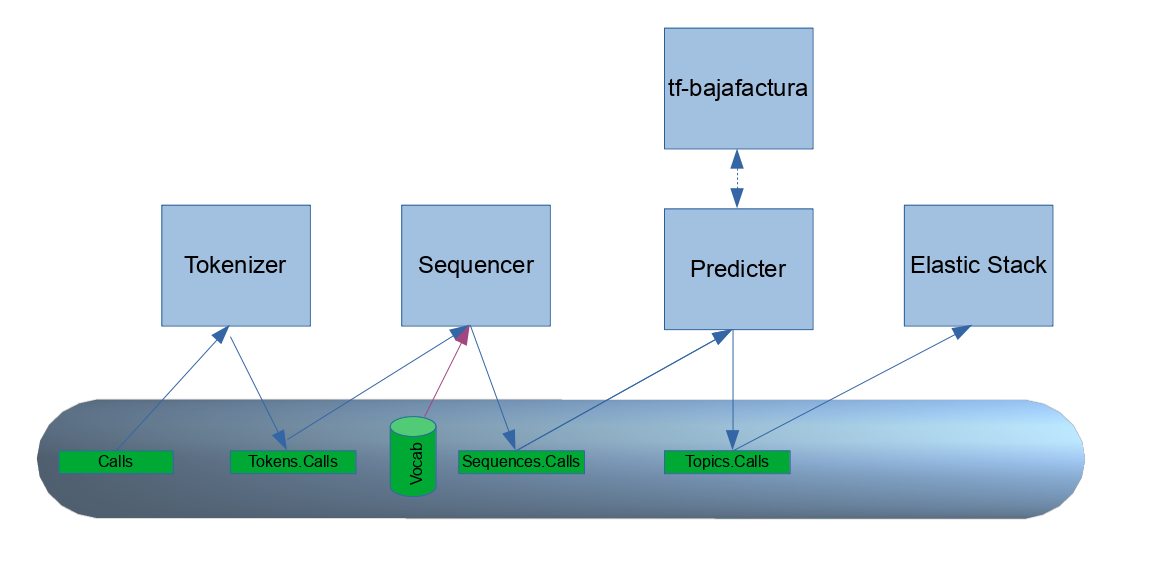
\includegraphics[width=1\textwidth]{images/exp/micro-arch}
	\caption{Arquitectura microservicios}
	\label{fig:micro-arch}
\end{figure}


En la figura \ref{fig:micro-arch} podemos ver como los microservicios propuestos interactúan entre sí a través del bus, con excepción del microservicio  \textbf{\textit{tf-BajaFactura}}. Estos microservicios conforman la parte capa de \textit{streaming} de nuestro sistema. En el capítulo siguiente veremos como la salida de esta capa de \textit{streaming} alimentará la capa de servicio.


A continuación, en los siguiente subapartados describiremos uno a uno los diferentes microservicios. 


\subsection{Tokenizer}

Este microservicio tiene como entrada las llamadas transcritas que llegan al bus en tiempo real. A partir del texto de las mismas el sistema inicia un proceso de \textit{tokenizacion} eliminando \textit{stopwords}, carácteres especiales (signos de puntuación, 'ñ's, acentos...), palabras comunes, números, nombres propios y pasando a minúscula cada uno de los tokens.  El proceso de \textit{tokenización} pretende ser lo más fiel posible al proceso realizado en \textit{Python} durante la etapa de entrenamiento del modelo.

Una vez obtenida la lista de \textit{tokens} esta se vuelve a disponibilizar en el bus en un nuevo \textit{topic}. Este nuevo \textit{topic} con las llamadas \textit{tokenizadas} puede ser de utilidad no solo para nuestro sistema, si no también para cualquier otro sistema de análisis de texto que necesite partir de los datos \textit{tokenizados}.

\subsection{Sequencer}
Este microservicio toma como entrada la salida del microservicio anterior y a partir de la lista de \textit{tokens} devuelve una secuencia de tamaño fijo determinado $T$. Para ello, utiliza un diccionario en el que cada \textit{token} se corresponde con un número, utilizando el $0$ para \textit{tokens} que no existan en este diccionario. Esta secuencia esta limitada a un tamaño determinado $T$ por lo que llamadas con un número mayor de $tokens$ son recortadas y se utiliza \textit{padding} por la izquierda para completar la secuencia de llamadas con un tamaño menor a $T$.

El diccionario ha sido calculado en conjunto de entrenamiento y contiene el vocabulario del modelo, este diccionario contiene como clave todos los \textit{tokens} posibles y como valores el identificador usado para cada \textit{token}. La lectura del mismo se realiza desde el mismo bus, utilizando un topic compacto sin límite de retención.

Una vez obtenida la secuencia de caracteres, esta se disponibiliza en un nuvo \textit{topic} del bus. Además de por nuestro sistema, este valor puede ser consumido por otros microservicios o sistemas que tengan como objetivo aplicar diferentes modelos a las secuencias obtenidas.


\subsection{tf-BajaFactura}
\textit{\textbf{tf-BajaFactura}} quizás sea el microservicio más tradicional y discordante de los que vamos a utilizar en nuestro sistema debido a que este microservicio se encuentra totalmente desacoplado del bus y del resto de microservicios. Mediante un \textit{API REST} aplica nuestro modelo de \textit{TensorFlow} a una o varias secuencia de entradas y, para cada secuencia, devuelve la probabilidad de pertenencia a las clases: ``Baja'', ``Factura'' y ``Resto''.

El motivo principal para usar \textit{API REST} en este microservicio se debe al uso de \textit{Tensorflow Serving} que nos permite con mucha facilidad desplegar nuevos modelos y algoritmos manteniendo la misma estructura en el servidor y la misma \textit{API}. Además su integración es automática con los modelos generados con \textit{TensorFlow} (con o sin \textit{Keras}). Esta decisión permite a los \textit{data-scientist} desplegar nuevas versiones de sus modelos ya sea por degradación o por mejora, mientras el resto del flujo permanece inalterable. 


\subsection{Predicter}
Este último microservicio tiene como entrada el \textit{topic} generado por \textit{\textbf{Sequencer}} y a partir del mismo realiza una llamada a \textit{\textbf{tf-BajaFactura}}. Una vez obtenidas las predicciones, las enriquece con las etiquetas necesarias. Además en el caso de existir un atributo de control comprueba si la predicción ha sido correcta, esto nos servirá para validar la eficiencia del modelo a lo largo del tiempo. 

Como podemos observar, es el único microservicio que tiene una dependencia con otro (\textit{tf-BajaFactura}), sin embargo la API de un modelo implementado con \textit{Tensorflow Serving}\cite{serving} es siempre idéntica por lo que la llamada no varía aunque cambie el modelo y el número de clases y las etiquetas de las mismas son configurables en \textit{\textbf{Predicter}} por lo que puede reutilizarse para cualquier servicio predictivo desplegado con  \textit{Tensorflow Serving}.

La salida de este microservicio es publicada en un nuevo \textit{topic} en el bus, esta información puede ser de utilidad para diversos sistemas que quieran realizar analítica en función de la temática de las llamadas o que quieran visualizarla. Nosotros la usaremos en nuestra capa de servicio que describiremos en el siguiente capítulo.


\section{Monitorización de Microservicios}

Si bien es cierto que el hecho de utilizar una arquitectura orientada a eventos, aparte de la sencillez intrínseca de nuestro sistema, nos simplifica en cierto modo la orquestación de nuestro servicios y nos permite prescindir de herramientas de APM (\textit{Application Performance Monitoring}); una monitorización del desempeño de nuestros microservicios es siempre necesaria, tanto para garantizar el correcto funcionamiento de los mismos y poder detectar posibles puntos de fallos como para detectar pérdidas de rendimiento en cualquier punto del sistema. 

En esta sección veremos los métodos utilizados para monitorizar los microservicios dependiendo de su tecnología. 


\subsection{Servicios \textit{Kafka Streams}}

Los servicios de Kafka Streams corren sobre la máquina virtual de Java lo que nos permite tener acceso a sus métricas por medio de la \textit{JMX}(\textit{Java Management Console}). Ademas \textit{Confluent} posee una documentación de los \textit{MBeans} y de las métricas que contienen en su documentación oficial \cite{Kafka Streamsmonitoring}. 


El inconveniente de estas métricas es que tienen que extraerse por medio de protocolos \textit{RMI}(\textit{Java Remote Method Invocation}) lo que complica su explotación, sin embargo a partir de la versión 6 del \textit{JDK} (\textit{Java Development Kit}) tenemos la posibilidad de exportar estas métricas de \textit{JMX} directamente mediante \textit{API REST}. Esto nos da la posibilidad de poder recolectar las métricas directamente mediante una llamada \textit{HTTP}.

Para recolectar estás métricas utilizaremos los \textit{Beats} de  \textit{Elastic}, concretamente \textit{Metricbeat}. Este será el encargado de recolectar las métricas necesarias y enviarlas a \textit{Logstash} para su posterior almacenamiento en \textit{Elasticsearch}. El flujo de \textit{Logstash} a \textit{Elasticsearch} lo trataremos con más detalle en el próximo capítulo en el que veremos la capa de servicio, ya que las métricas de monitorización seguirán el mismo recorrido que los datos de clasificación. 


De todas las métricas disponibles de Confluent, nosotros extraeremos con una frecuencia de un minuto las siguientes métricas:

\begin{itemize}
	\item \textit{mbean 'java.lang:type=Runtime'} : Métrica \textit{Uptime}.
	
	\item \textit{mbean 'kafka.streams:type=stream-metrics'}: Métricas \textit{process-latency-avg}, \textit{process-latency-max} y \textit{process-rate}.
\end{itemize}



Esto nos permitirá para cada microservicio tener información del tiempo de servicio del mismo, de la latencia máxima y media de procesamiento de los eventos y de la tasa de procesamiento. 





\subsection{Servicios \textit{Tensorflow Serving}}

En el caso de la monitorización del servicio \textit{tf-BajaFactura}, habilitaremos la monitorización de \textit{Prometheus} de \textit{Tensorflow Serving} para que las métricas sean accesibles mediante \textit{API REST}, pero en lugar de utilizar \textit{Prometheus} (para no incluir complejidad en nuestro sistema), usaremos directamente el \textit{Input} \textit{Http\_poller} de \textit{Logstash}.

De todas las métricas disponibles en \textit{Tensorflow Serving} nos quedaremos unicamente con: 

\begin{itemize}
\item \textbf{Estado}: Que nos dará información sobre si el modelo está operativo.  

\item \textbf{Total peticiones}: Total de peticiones resueltas por el modelo.

\item \textbf{Total nanosegundos del grafo}: El total de tiempo que el modelo ha dedicado en procesar todas las peticiones. Utilizaremos el total de peticiones para extraer la latencia media y lo expresaremos en milisegundos. 

\end{itemize}




Una vez recolectadas las métricas en \textit{Logstash}, seguirán el mismo flujo descrito en el apartado anterior que veremos en más detalle en el apartado siguiente. 

Además de las métricas recolectadas, la monitorización del microservicio \textit{\textbf{predicter}} nos dará información combinada de ambos ya que internamente realiza una llamada a \textit{tf-BajaFactura}.



\section{Inyector: simulador de tiempo real}
Como ya hemos comentado en anteriores capítulos actualmente las transcripciones de las llamadas no se encuentran disponible en tiempo real, es por ello que se ha diseñado un inyector de llamadas.

Este inyector, realizado en \textit{Python} utiliza como fuente la transcripción de las llamadas realizadas en batch. Y a partir de la misma cumplirá los siguientes objetivos: 

\begin{itemize}
	\item \textbf{ Extraer la frecuencia de llamadas por hora}. De este modo simularemos el comportamiento real de un \textit{call-center} inyectando más llamadas a las horas de mayor actividad.
	\item \textbf{Multiplicar el número de llamadas}. Teniendo en cuenta que actualmente solo se transcriben un 4\% del total de las llamadas, el inyector multiplicará por 25 el número de llamadas recibidas en un día para simular el comportamiento real de un sistema que transcriba el 100\% de las llamadas.
	\item \textbf{Introducir datos de control}: El inyector insertará en un porcentaje de llamadas los datos reales de clasificación con el fin de poder verificar el comportamiento del modelo. En un entorno real se podrían insertar periódicamente un número de llamadas de control que nos permitan este objetivo.
	
\end{itemize}

Una vez realizadas estas tareas, el inyector publicará todas las llamadas al bus, simulando un comportamiento real. De este modo las llamadas estarán disponibles en tiempo real para cualquier consumidor que las necesite.

Aunque el inyector podría verse como un microservicio más, hemos preferido dejarlo fuera del sistema a lo largo de todo el apartado, debido a que lo consideramos una pieza auxiliar que nos permite simular el comportamiento real del sistema sin disponer de los datos en este momento.


\chapter{Capa de servicio}


\section{Carga y modelo}


\section{Visualizaciones}

\subsection{Monitorización}
\subsection{Sistema}

\section{Alarmado}





\chapter{Despliegue en contenedores}
Una vez desarrollados los microservicios y su monitorización, es necesario ponerlos en producción, y una de las decisiones importantes es donde queremos que corran si en máquinas físicas, máquinas virtuales o en contenedores (en nuestro caso, se descarta la opción de implementarlo en \textit{Cloud}). La decisión tomada es que todo corra sobre contenedores en una plataforma \textit{\textbf{OCP}} \textit{Openshift Container Platform}, los motivos de esta decisión son los siguientes: 

\begin{itemize}
	\item \textit{\textbf{Stateless}}: Todos los servicios implementado no necesitan estado (los datos necesarios se almacenan en el bus). Lo que lo hace un caso de uso ideal para su ejecución en contenedores. 
	\item \textbf{Agilidad de despliegue}: El proceso de creación y destrucción de un contenedor es inmediato, lo que no da mucha flexibilidad a la hora desplegar nuevos contenedores.
	
	\item \textbf{Serivicios Autocontenidos}: Los contenedores pueden ejecutarse en multitud de plataforma lo que nos permite tener aplicaciones inmutables y autocontenidas que podemos mover entre plataformas y entornos. Este punto y el anterior serán de mucha utilidad a la hora de implementar la integración y el despliegue continuo.
	
	\item  \textbf{Alta disponibilidad}: Al tener un clúster de \textit{Openshift} con múltiples nodos, en el caso que se produjera un fallo en un nodo que provocará la caída de un contenedor, este se levantaría automáticamente en otro nodo. 
	
\end{itemize} 

A la largo del apartado nos referiremos a los siguientes conceptos propios de \textit{Openshift} (muchos de ellos heredados en \textit{Kubernetes}):

\begin{itemize}
\item  \textit{\textbf{Pod}}: Un pod es la unidad mínima en \textit{OCP}. Puede estar formado por uno o varios contenedores (\textit{Docker}), pero todos ellos correran en una única máquina y tendrán una única dirección IP.

\item  \textit{\textbf{Despliegue}}: Un despliegue (\textit{Deployment}) pordemos decir, de una manera muy simplificada, que gestiona el número de réplicas de un pod. 

\item  \textbf{Configuración de despliegue}: La configuración de despliegue (\textit{Deployment Config}) dota a los despliegues de un ciclo de vida proporcionando versiones de los mismo, disparadores para crear nuevos despliegues de manera automática y estrategias para realizar transiciones entre diferentes versiones de despliegues sin pérdida de servicio. 

\item  \textbf{Servicio}: Un servicio expone un número determinado de Pods para que sean accesibles desde otros elementos de la plataforma. 

\item  \textbf{\textit{ConfigMap}}: Se trata de un mecanismo de \textit{OCP} para almacenar elementos de configuración mediante un mecanismo de clave-valor. Es posible almacenar tanto ficheros como valores simples.


\end{itemize}

\begin{figure}[!ht]
	\centering
	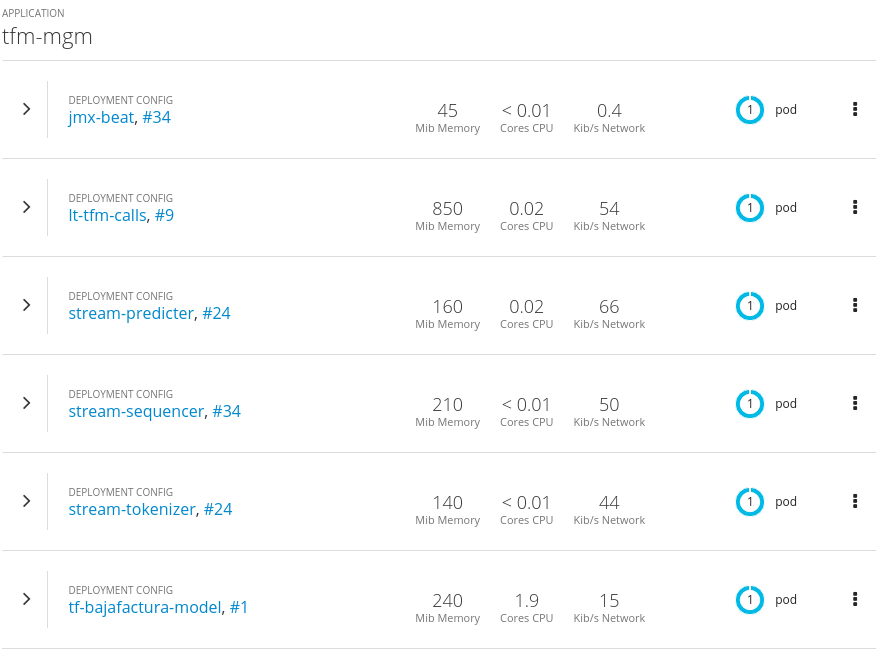
\includegraphics[width=1\textwidth]{images/cont/overview}
	\caption{configuración de despliegue y recursos usados en OCP}
	\label{fig:ocp-overview}
\end{figure}

En la figura \ref{fig:ocp-overview} podemos ver las diferentes configuraciones de despliegue con los \textit{pods} que tienen levantados cada uno y los recursos de memoria, cpu y red que consumen cada uno. 
 
A continuación veremos un resumen de los servicios, despliegues y configuraciones desplegadas en Openshift para cada tipo de microservicio y monitorización. En el apéndice \cite{apendi:contenedores} podemos encontrar todo el código de despliegue en Openshift, que nos permitiría desplegar todo nuestro entorno en otro clúster en cuestión de minutos. 


\section{Servicios \textit{Kafka Streams}}

Para desplegar los servicios de \textit{Kafka Streams} en \textit{OCP} es necesario desplegar un configuración de despliegue por microservicio, un servicio para exponer las métricas y disponer en un \textit{configmap} de las opciones necesarias para su ejecución. 

En este apartado únicamente presentaremos a modo de ejemplo el configuración de despliegue y el servicio  del microservicio \textit{Predicter} explicando las características más relevantes del mismo. Tanto el \textit{configmap} con todos los ficheros como el resto de despliegues pueden consultarse en el apéndice \cite{apendi:contenedores}. 

El configuración de despliegue de \textit{Predicter} es el siguiente: 

\begin{minted}[
	gobble=0,
	frame=single,
	linenos
	]{yaml}

apiVersion: apps.openshift.io/v1
kind: DeploymentConfig
metadata:
  labels:
    app: tfm-mgm
    project: topic-model
    service: stream-predicter
  name: stream-predicter
  namespace: nbia-prod
spec:
  replicas: 1
  revisionHistoryLimit: 10
  selector:
    deploymentconfig: stream-predicter
  strategy:
    activeDeadlineSeconds: 21600
    recreateParams:
      timeoutSeconds: 600
    resources: {}
    type: Recreate
  template:
    metadata:
      creationTimestamp: null
      labels:
        app: tfm-mgm
        deploymentconfig: stream-predicter
        project: topic-model
        service: calls-predicter
    spec:
      containers:
        - env:
            - name: JAVA_MAIN_CLASS
              value: com.telefonica.topicmodel.PredicterLauncher
          image: >-
            docker-registry.default.svc:5000/nbia-prod/
            topic-model-streaming:latest
          imagePullPolicy: Always
          name: stream-predicter
          ports:
            - containerPort: 8778
              protocol: TCP
          resources:
            limits:
              cpu: '1'
              memory: 512Mi
            requests:
              cpu: 200m
              memory: 256Mi
          terminationMessagePath: /dev/termination-log
          terminationMessagePolicy: File
          volumeMounts:
            - mountPath: /opt/jolokia/etc/jolokia.properties
              name: calls-config
              subPath: jolokia.properties
            - mountPath: /deployments/application.json
              name: calls-config
              subPath: topic-model-streaming.json
      dnsPolicy: ClusterFirst
      restartPolicy: Always
      schedulerName: default-scheduler
      terminationGracePeriodSeconds: 30
      volumes:
        - configMap:
            defaultMode: 420
            name: calls-config
          name: calls-config
  test: false
  triggers:
    - imageChangeParams:
        automatic: true
        containerNames:
          - stream-predicter
        from:
          kind: ImageStreamTag
          name: 'topic-model-streaming:latest'
          namespace: nbia-prod
      type: ImageChange
    - type: ConfigChange

\end{minted}

Del despliegue anteriormente expuesto podemos destacar las siguientes características: 

\begin{itemize}
	\item \textbf{labels} (línea 4):  Nos ayudan a identificar el despliegue, el proyecto y la aplicación. Todos los despliegues relacionados con el TFM que se presenta en este documento tendrán el indicador \textit{tfm-mgm}. 

	\item \textbf{replicas} (línea 11): Indica el número de réplicas de cada \textit{Pod} que pueden correr al mismo tiempo. En este caso lo establecemos a uno, pero podría escalar horizontalmente incluso hacerlo de manera automática por uso de CPU o memoria mediante un \textit{Horizontal Pod Autoscaler}. 


	\item \textbf{replicas} (línea 11): Indica el número de réplicas de cada \textit{Pod} que pueden correr al mismo tiempo. En este caso lo establecemos a uno, pero podría escalar horizontalmente incluso hacerlo de manera automática por uso de CPU o memoria mediante un \textit{Horizontal Pod Autoscaler}. 

	\item \textbf{strategy} (línea 15): Establecemos la estrategia con la que se implantará una nueva versión del \textit{deployment}, en este caso utilizamos una estrategia \textit{Recreate} que para todos los servicios de un \textit{deployment} anterior antes de iniciar uno nuevo. Debido a que el bus tiene capacidad de retención de los eventos esto no implicará una interrupción en el servicio, si no un ligero retraso en el momento del despliegue.

	\item \textbf{Container} (línea 30): Aquí encontramos toda la información del del contenedor que se desplegará. Destacamos: 
		\begin{itemize}
			\item \textbf{env} (línea 31): Variables globales del \textit{deploynment}, en este caso la clase Java  principal que se lanzará al ejecutar el contenedor. 
			\item \textbf{image} (línea 34): Contiene la referencia a la imagen del contenedor que queremos desplegar. Se trata de una imagen de Java con nuestro código que se encuentra almacenada en el repositorio de la plataforma. El parámetro \textit{imagePullPolicy} indica en que circunstancias se descargará la imagen del repositorio (en este caso lo hará siempre, exista o no en el nodo en el que se despliega el \textit{Pod}).
			\item \textbf{Ports} (línea 34): Indica los puertos que expondrá el contenedor, en este caso se expondrá unicamente el puerto 8778 que es el puerto por defecto del \textit{endpoint} de \textit{Jolokia}.
			\item \textbf{Resources} (línea 42): Contiene los recursos de CPU y memoria que solicitará el \textit{Pod}  al arrancar y a los que estara limitados. 
			\item \textbf{VolumeMounts} (línea 51): Indica los volúmenes que montará el contenedor, en este caso son todos procedentes de un \textit{configmap} y contienen los ficheros de configuración de \textit{jolokia} y de la aplicación.
		\end{itemize}
	\item  \textbf{volumes} (línea 62): Contiene los volúmenes que se utilizaran en los contenedores en el apartado \textit{VolumeMounts}. En este caso unicamente contiene un \textit{configmap}. 
	\item \textbf{triggers} (línea 68): Define los disparadores que provocaran que se realice un nuevo \textit{deployment}, en este caso la modificación de la imagen o la modificación del configuración de despliegue.

\end{itemize}


El servicio de \textit{Predicter} es el siguiente: 

\begin{minted}[
	gobble=0,
	frame=single,
	linenos
	]{yaml}

apiVersion: v1
kind: Service
metadata:
  labels:
    app: tfm-mgm
  name: stream-predicter
  namespace: nbia-prod
spec:
  ports:
    - name: 8778-tcp
      port: 8778
      protocol: TCP
      targetPort: 8778
  selector:
    deploymentconfig: stream-predicter
  sessionAffinity: None
  type: ClusterIP

\end{minted}

Aparte de las etiquetas que tienen las misma utilidad que el configuración de despliegue visto anteriormente, cabe destacar los siguiente parámetros: 

\begin{itemize}
	\item \textbf{name} (línea 6): El nombre del servicio que usaremos para llamarlo dentro de la plataforma. 
	 \item \textbf{name} (línea 6):
	 \item \textbf{ports} (línea 9): El puerto que expondrá el servicio y al puerto de los \textit{pods} que atacará. 
	 \item \textbf{selector} (línea 14): Los \textit{pods} a los que atacará el servicio. En este caso los \textit{pods} pertenecientes al configuración de despliegue \textit{stream-predicter}. 
	 
	 \item \textbf{sessionAffinity} (línea 16): Si quisieramos establecer alguna afinidad, por ejemplo a nivel de \textit{IP}, para que un mismo origen ataque siempre a un mismo \textit{Pod}. Hay que recordar que los servicios en \textit{Openshift} (y \textit{Kubernetes}) actuan como un balanceador entre los \textit{pods}.
\end{itemize}




\section{Servicios \textit{Tensorflow Serving}}

En el caso del servicio de TensorflowServing mostraremos solo la configuración de despliegue aunque también consta de un servicio para que podamos realizar llamadas \textit{HTTP} sobre el mismo desde la plataforma de \textit{Openshift}. En el caso de que se quisiera acceder al servicio desde fuera de la plataforma será necesario recurrir las \textit{Routes} de Openshift.

La configuración de despliegue de \textit{tf-BajaFactura} es el siguiente:

 
\begin{minted}[
	gobble=0,
	frame=single,
	linenos
	]{yaml}
apiVersion: apps.openshift.io/v1
kind: DeploymentConfig
metadata:
  labels:
    app: tfm-mgm
    appName: tf-bajafactura-model
    appTypes: tensorflow-serving-s2i
    appid: tf-serving-tf-bajafactura-model
  name: tf-bajafactura-model
  namespace: nbia-prod
spec:
  replicas: 1
  revisionHistoryLimit: 10
  selector:
    deploymentconfig: tf-bajafactura-model
  strategy:
    activeDeadlineSeconds: 21600
    rollingParams:
      intervalSeconds: 1
      maxSurge: 25%
      maxUnavailable: 25%
      timeoutSeconds: 600
      updatePeriodSeconds: 1
    type: Rolling
  template:
    metadata:
      labels:
        app: tfm-mgm
        appName: tf-bajafactura-model
        appTypes: tensorflow-serving-s2i
        appid: tf-serving-tf-bajafactura-model
        deploymentconfig: tf-bajafactura-model
    spec:
      containers:
        - env:
            - name: PORT
              value: '8501'
            - name: MODEL_NAME
              value: bajafactura
            - name: RUN_OPTIONS
          image: >-
            docker-registry.default.svc:5000/nbia-prod/
            tf-bajafactura-model:latest
          imagePullPolicy: Always
          livenessProbe:
            failureThreshold: 10
            httpGet:
              path: /v1/models/bajafactura
              port: 8501
              scheme: HTTP
            initialDelaySeconds: 20
            periodSeconds: 30
            successThreshold: 1
            timeoutSeconds: 5
          name: tf-bajafactura-model
          ports:
            - containerPort: 8501
              protocol: TCP
          readinessProbe:
            failureThreshold: 1
            httpGet:
              path: /v1/models/bajafactura
              port: 8501
              scheme: HTTP
            initialDelaySeconds: 20
            periodSeconds: 10
            successThreshold: 1
            timeoutSeconds: 5
          resources:
            limits:
              cpu: '2'
              memory: 2Gi
            requests:
              cpu: '1'
              memory: 1Gi
          terminationMessagePath: /dev/termination-log
          terminationMessagePolicy: File
      dnsPolicy: ClusterFirst
      restartPolicy: Always
      schedulerName: default-scheduler
      terminationGracePeriodSeconds: 30
  test: false
  triggers:
    - imageChangeParams:
        automatic: true
        containerNames:
          - tf-bajafactura-model
        from:
          kind: ImageStreamTag
          name: 'tf-bajafactura-model:latest'
          namespace: nbia-prod
      type: ImageChange
    - type: ConfigChange


\end{minted}

En este caso solo comentaremos los parámetros que varían con respecto al despliegue de los servicios \textit{Kafka Streams}: 
\begin{itemize}
	\item \textbf{strategy} (línea 16): En este caso la estrategia en el caso de que exista un nuevo despliegue se denomina \textit{Rolling}. Esto implica, de forma muy resumida, que el nuevo \textit{deployment} se hará de manera paulatina, no eliminando los \textit{deployment} anteriores hasta que no se hayan realizado los nuevos. Esto garantiza que no exista una pérdida de servicio en los nuevos despliegues.  
	\item \textbf{image} (línea 41): La imagen usada en este caso es la imagen de \textit{docker} de \textit{TensorFlow Serving} con nuestro modelo cargado que se encuentra almacenada en el repositorio de la plataforma.
	\item \textbf{livenessProbe} (línea 45): Comprueba que el contenedor sigue con vida, de no ser así durante el número de intentos establecido se reiniciará el contenedor. En este caso la comprobación es una petición \textit{HTTP} al \textit{endpoint} de estado del modelo.
	 \item \textbf{readinessProbe} (línea 59): Antes de enviar tráfico a un \textit{pod}, este debe estar en estado \textit{ready}. Con este parámetro establecemos que el \textit{pod} no se encuentre \textit{ready} hasta que no se haya verificado el \textit{endpoint} de estado del modelo.
\end{itemize}

Aunque existen otros parámetros que varian como las variables de entornos o los recursos definidos el funcionamiento es igual al configuración de despliegue definido anteriormente.


\section{Monitorización}

Los despliegues vistos hasta ahora nos permiten tener funcionando nuestro sistema, sin embargo, no debemos olvidarnos de la monitorización necesaria, que ya describimos en el capítulo \ref{chapter:prod}, para verificar el correcto funcionamiento del mismo. 

Dentro de Openshift la monitorización esta formada por dos despliegues diferentes:

\begin{itemize}
\item \textbf{Logstash}: Podemos identificarlo en la figura \ref{fig:ocp-overview} con el nombre \textbf{lt-tfm-calls} y será el encargado de llevar a la capa de servicio no solo la monitorización de todo el sistema, si no también los datos de clasificación de llamadas y  de realizar las transformaciones necesarias. 

\item \textbf{Metricbeat}: Podemos identificarlo en la figura \ref{fig:ocp-overview} con el nombre \textbf{jmx-beat} y será el encargado de extraer las métricas de Jolokia de los servicios de \textit{Kafka Streams}. 
\end{itemize}

A continuación veremos la configuración de ambos despliegues.

\subsection{Logstash}
Al igual que en los casos anteriores, vemos unicamente la configuración del despliegue, pudiendo encontrar el resto de recursos en el anexo \ref{anexo}. 

La configuración de despliegue es la siguiente:

\begin{minted}[
 	gobble=0,
 	frame=single,
 	linenos]{yaml}
apiVersion: apps.openshift.io/v1
kind: DeploymentConfig
metadata:
  labels:
    app: tfm-mgm
    service: lt-tfm-calls
    version: '1.0'
  name: lt-tfm-calls
  namespace: nbia-prod
spec:
  replicas: 1
  revisionHistoryLimit: 10
  selector:
    deploymentconfig: lt-tfm-calls
  strategy:
    activeDeadlineSeconds: 21600
    resources: {}
    rollingParams:
      intervalSeconds: 1
      maxSurge: 25%
      maxUnavailable: 25%
      timeoutSeconds: 600
      updatePeriodSeconds: 1
    type: Rolling
  template:
    metadata:
      labels:
        app: tfm-mgm
        deploymentconfig: lt-tfm-calls
        service: lt-tfm-calls
        version: '1.0'
    spec:
      containers:
        - env:
            - name: PIPELINE
              value: tfm-calls
            - name: LS_JAVA_OPTS
              value: '-Xmx2g'
            - name: USER_LOGSTASH
              valueFrom:
                secretKeyRef:
                  key: username
                  name: logstash-internal-user
            - name: PASS_LOGSTASH
              valueFrom:
                secretKeyRef:
                  key: password
                  name: logstash-internal-user
          image: 'docker-registry.default.svc:5000/openshift/logstash:7.4.2'
          imagePullPolicy: IfNotPresent
          livenessProbe:
            failureThreshold: 10
            httpGet:
              path: /
              port: 9600
              scheme: HTTP
            initialDelaySeconds: 300
            periodSeconds: 30
            successThreshold: 1
            timeoutSeconds: 5
          name: lt-tfm-calls
          ports:
            - containerPort: 5010
              protocol: TCP
            - containerPort: 9600
              protocol: TCP
          readinessProbe:
            failureThreshold: 1
            httpGet:
              path: /
              port: 9600
              scheme: HTTP
            initialDelaySeconds: 120
            periodSeconds: 10
            successThreshold: 1
            timeoutSeconds: 5
          resources:
            limits:
              cpu: '1'
              memory: 2200Mi
            requests:
              cpu: 500m
              memory: 2Gi
          terminationMessagePath: /dev/termination-log
          terminationMessagePolicy: File
          volumeMounts:
            - mountPath: /usr/share/logstash/config/logstash.yml
              name: calls-config
              subPath: logstash.yml
      dnsPolicy: ClusterFirst
      restartPolicy: Always
      schedulerName: default-scheduler
      terminationGracePeriodSeconds: 30
      volumes:
        - configMap:
            defaultMode: 420
            name: calls-config
          name: calls-config
  test: false
  triggers:
    - type: ConfigChange
 
\end{minted}

 Algunas características que podemos observar diferentes a las vistas actualmente son: 
 
 \begin{itemize}
 \item \textit{Secrets} (líneas 40 y 45): En este despliegue vemos que las variables globales para la autenticación se cargan de un recurso de \textit{OCP} denominado \textit{Secret}, utilizado para almacenar información sensible.
 \item  \textit{\textbf{image}} (línea 49): En este caso la imagen no contiene ningún código propio como en resto de despliegues vistos anteriormente. Se trata de la imagen oficial de \textit{Elastic}. El código a ejecutar (\textit{pipeline}) se almacena de forma centralizada en \textit{Elasticsearch} y utilizamos la variable de entorno \textit{PIPELINE} y los ficheros de configuración (\textit{configmaps}) para acceder a la información. 
 \item \textit{\textbf{resources}} (línea 77): En este caso vemos que los recursos solicitados son mayores que en el resto de despliegues. Esto se debe a que el \textit{Heap} que tiene configurado la imagen de \textit{Logstash} por defecto es mayor, podría modificarse para optimizar el uso de recursos, pero no hemos tenido esa necesidad.
 \end{itemize}



\subsection{Metricbeat}

El último despliegue que nos queda por ver, es probablemente el más simple, el de \textit{Metricbeat}, el agente encargado de extraer las métricas de \textit{Jolokia} de los servicios de  \textit{Kafka Streams}. Este despliegue no tiene asociado ningún servicio, ya que no será llamado por otros componentes. 

La configuración de despliegue de \textit{Metricbeat} es la siguiente: 

\begin{minted}[
 	gobble=0,
 	frame=single,
 	linenos]{yaml}
apiVersion: apps.openshift.io/v1
kind: DeploymentConfig
metadata:
  labels:
    app: tfm-mgm
    deploymentconfig: jmx-beat
    service: jmx-beat
  name: jmx-beat
  namespace: nbia-prod
spec:
  replicas: 1
  selector:
    deploymentconfig: jmx-beat
  strategy:
    activeDeadlineSeconds: 21600
    resources: {}
    rollingParams:
      intervalSeconds: 1
      maxSurge: 25%
      maxUnavailable: 25%
      timeoutSeconds: 600
      updatePeriodSeconds: 1
    type: Rolling
  template:
    metadata:
      labels:
        app: tfm-mgm
        deploymentconfig: jmx-beat
        project: tfmmgm
        service: jmx-beat
    spec:
      containers:
        - env:
            - name: ELASTICSEARCH_USERNAME
              valueFrom:
                secretKeyRef:
                  key: username
                  name: logstash-internal-user
            - name: ELASTICSEARCH_PASSWORD
              valueFrom:
                secretKeyRef:
                  key: password
                  name: logstash-internal-user
          image: >-
            docker-registry.default.svc:5000/nbia-prod/metricbeat:7.4.2
          imagePullPolicy: Always
          name: jmx-beat
          resources:
            limits:
              cpu: '1'
              memory: 512Mi
          terminationMessagePath: /dev/termination-log
          terminationMessagePolicy: File
          volumeMounts:
            - mountPath: /usr/share/metricbeat/metricbeat.yml
              name: calls-config
              subPath: metricbeat.yml
            - mountPath: /usr/share/metricbeat/modules.d/jolokia.yml
              name: calls-config
              subPath: jolokia.yml
      dnsPolicy: ClusterFirst
      restartPolicy: Always
      schedulerName: default-scheduler
      terminationGracePeriodSeconds: 30
      volumes:
        - configMap:
            defaultMode: 292
            name: calls-config
          name: calls-config
  test: false
  triggers:
    - type: ConfigChange
    - imageChangeParams:
        automatic: true
        containerNames:
          - jmx-beat
        from:
          kind: ImageStreamTag
          name: 'metricbeat:7.4.2'
          namespace: nbia-prod
      type: ImageChange
\end{minted}

Todos los parámetros vistos en este despliegue deberían resultarnos ya familiares. La imagen de \textit{docker} usada en este caso también se trata de la imagen oficial desarrollada por \textit{Elastic}.


\section{S2I}
Los despliegues en \textit{OCP} descritos a lo largo de este capítulo podrían clasificarse en dos: Aquellos que son imágenes oficiales con alguna configuración propia y aquellos que contienen código fuente o binarios propios. En el primer grupo se encuentra el agente \textit{Metricbeat} y \textit{Logstash} (aunque ejecuta código propio no está almacenado en la imagen), mientras que al segundo grupo pertenecen los microservicios de \textit{Kafka Streams} y el modelo de \textit{Tensorflow Serving}. A partir de ahora, nos centraremos en este segundo grupo.

La opción más simple para tener una imagen con nuestro código sería generarlas de forma individual y subirlas al repositorio de imágenes de la plataforma, sin embargo esta tarea se volvería algo tediosa conforme el número de servicios crezca, además presentaría dificultades en su mantenimiento y en su integración (como veremos más adelante) con flujos de integración y despliegue continuos. Es por eso que utilizaremos una característica de \textit{OCP} denominada \textit{S2I} (\textit{Sorce to Image}), que nos permitirá a partir de una imagen base (a partir de ahora imagen S2I) generar una nueva imagen personalizada con nuestra aplicación. 

El proceso de crear la imagen de nuestra aplicación a partir de una imagen S2I y nuestro código o binarios se denomina \textit{Build} y al igual que con la configuración de despliegue para los despliegues \textit{Openshift} nos proporciona una configuración de \textit{Build} para controlar las versiones y los cambios que se realizan en un mismo tipo de \textit{Build}. A continuación veremos como hemos abordado los casos de \textit{Kafka Streams} y \textit{Tensorflow Serving}.


\subsection{\textit{Kafka Streams}}

En este caso tenemos dos opciones a la hora de crear nuestra imagen de aplicación mediante S2I, partir del código fuente o partir de un binario (un jar generado a partir del código fuente). Hemos optado por esta segunda opción para dejar la compilación y tests fuera de la plataforma \textit{OCP}. 

La imagen \textit{S2I} utilizada es la imagen oficial proporcionada por RedHat para Java. Y a continuación podemos ver como quedaría nuestra configuración de \textit{Build}:

\begin{minted}[
 	gobble=0,
 	frame=single,
 	linenos]{yaml}
apiVersion: build.openshift.io/v1
kind: BuildConfig
metadata:
  labels:
    app: tfm-mgm
  name: topic-model-streaming
  namespace: nbia-prod
spec:
  failedBuildsHistoryLimit: 5
  output:
    to:
      kind: ImageStreamTag
      name: 'topic-model-streaming:latest'
  runPolicy: Serial
  source:
    binary: {}
    type: Binary
  strategy:
    sourceStrategy:
      from:
        kind: ImageStreamTag
        name: 'redhat-openjdk18-openshift:1.4'
        namespace: openshift
    type: Source
  triggers: []
\end{minted}

Algunos aspectos relevantes de la configuración de \textit{Build} son:

\begin{itemize}
\item \textit{\textbf{output}} (línea 10): Nos indica la imagen destino de aplicación que se creará. En nuestro caso la imagen es común ya que todas las clases están embebidas en un mismo binario, por eso posee un valor fijo, pero podría tener un valor variable. La imagen destino debe estar definida en la plataforma. 

\item \textit{\textbf{from}} (línea 20): La imagen \textit{S2I} que se utilizará para crear la imagen de aplicación.

\item \textit{\textbf{triggers}} (línea 25): Al tratarse de un \textit{S2I} binario no existen disparadores por lo que el \textit{Build} debe iniciarse de forma externa proporcionando los binarios.
 
\end{itemize}


\subsection{\textit{Tensorflow Serving}}

En este caso no tenemos elección entre realizar el \textit{build} con fuente o binario, debido a que los modelos que tenemos de \textit{Tensorflow} son binarios. La aproximación, por tanto, será la misma que en el apartado anterior. 

Sin embargo, en este caso no existe ninguna imagen oficial S2I para \textit{Tensorflow Serving} por lo que nos hemos visto obligados a crear nuestra propia imagen S2I a partir de la imagen oficial de \textit{docker} de \textit{Tensorflow Serving}.

El proceso de creación de una imagen S2I consta, a grandes rasgos, de los siguientes pasos: 

\begin{itemize}
\item \textit{Assemble}: Crear los scripts necesarios para una vez recibido los ficheros colocarlos en la ruta adecuada y construir con ellos la imagen de aplicación. 
\item \textit{run}: Establecer como debe comportarse la imagen de aplicación.
\item \textit{usage}: Recopilar el modo de uso de la imagen S2I. 

\end{itemize}

Todo el código de creación de la imagen así como el build de \textit{Tensorflow Serving} (practicamente idéntico al anterior) puede encontrarse en el anexo \ref{anexo}.






\part{Conclusiones: mantenimiento y futuros trabajos }

% bibliografia
\addcontentsline{toc}{chapter}{Bibliografía}
\bibliographystyle{plain}
\bibliography{referencias}

\end{document}